\documentclass[sigconf, nonacm]{acmart}
%% The following content must be adapted for the final version
% paper-specific
\newcommand\vldbdoi{XX.XX/XXX.XX}
\newcommand\vldbpages{XXX-XXX}
% issue-specific
\newcommand\vldbvolume{14}
\newcommand\vldbissue{1}
\newcommand\vldbyear{2020}
% should be fine as it is
\newcommand\vldbauthors{\authors}
\newcommand\vldbtitle{\shorttitle} 
% leave empty if no availability url should be set
\newcommand\vldbavailabilityurl{}
% whether page numbers should be shown or not, use 'plain' for review versions, 'empty' for camera ready
\newcommand\vldbpagestyle{plain} 


%\newcommand{\red}{\textcolor{red}}
\newcommand{\techreport}{our technical report~\cite{techreport}}
\newcommand{\titlename}{Systems for Large-Model Deep Learning Training}
% eat only in tech reports
\newcommand{\techreporteat}{}


\usepackage{hyperref,array,color,balance,multirow}
\usepackage{balance,float,url,amsfonts,alltt}
\usepackage{mathtools,rotating,amsmath}

\usepackage{etoolbox,listings}
\lstset{basicstyle=\ttfamily\tiny,breaklines=true}
\usepackage{bigstrut,morefloats,pbox}
\usepackage{graphicx,subfigure,xspace,verbatim,comment}
\usepackage{grffile}
\usepackage{ifpdf,fancyvrb}
\usepackage{algorithm}
\usepackage[noend]{algorithmic}
\usepackage{booktabs}
\usepackage{lipsum}  
\usepackage[all]{nowidow}
\usepackage{multirow}
\usepackage{pifont}
\usepackage{xcolor}

\newtheorem{theorem}{Theorem}[section]
\newtheorem{proposition}{Proposition}[section]
\newtheorem{corollary}[theorem]{Corollary}
\newtheorem{lemma}[theorem]{Lemma}
\newtheorem{definition}{Definition}[section]
\newcommand{\eat}[1]{}
 \newcommand{\eqdef}{=\mathrel{\mathop:}}
 \definecolor{mygreen}{HTML}{3EC300}
\newcommand\red[1]{\textbf{\color{red}#1}}
\newcommand{\xmark}{\color{red} \ding{55}}%

\DeclareMathOperator*{\gammasum}{\scalerel*{\Gamma}{\sum}}
\usepackage{scalerel}

%\DeclarePairedDelimiter{\ceil}{\lceil}{\rceil}

\newenvironment{packeditems}{
\begin{itemize}
  \setlength{\itemsep}{1pt}
  \setlength{\parskip}{0pt}
  \setlength{\parsep}{0pt}
}{\end{itemize}}

\newenvironment{packedenums}{
\begin{enumerate}
  \setlength{\itemsep}{1pt}
  \setlength{\parskip}{0pt}
  \setlength{\parsep}{0pt}
}{\end{enumerate}}

%\newcolumntype{P}[1]{>{\centering\arraybackslash}p{#1}}

\newtoggle{TR}
%\toggletrue{TR}

\DeclareMathOperator*{\argmin}{arg\,min}


\begin{document}\sloppy
\title{\titlename}



%\numberofauthors{8}
\author{Kabir Nagrecha}
\affiliation{%
\institution{University of California, San Diego}
}
\email{knagrech@ucsd.edu}



\begin{abstract}
Deep learning has transformed applications in a variety of domains, including computer vision, natural language processing, and tabular data analysis. The search for improved deep learning model accuracy has led practitioners to explore
increasingly larger model architectures, with some recent Transformer architecture designs using hundreds of billions of learnable parameters. The scale of these model architectures has introduced new systems challenges such as memory 
bottlenecks, poor runtime efficiency, and excessive computational costs of model development. Efforts to address these issues have explored techniques such as parallelization of neural architectures, spilling data across the memory hierarchy, and model compression. This survey will explore some key systems that incorporate these techniques, and evaluate their effectiveness in supporting large-model training. 
\end{abstract}
\maketitle

\pagestyle{\vldbpagestyle}
\techreporteat{
%%% do not modify the following VLDB block %%
%%% VLDB block start %%%
%%% VLDB block end %%%

%%% do not modify the following VLDB block %%
%%% VLDB block start %%%
\vspace{.3cm}
}
%%% VLDB block end %%%




\section{Introduction}
\label{sec:intro}
\begin{figure}[t]
 \centering
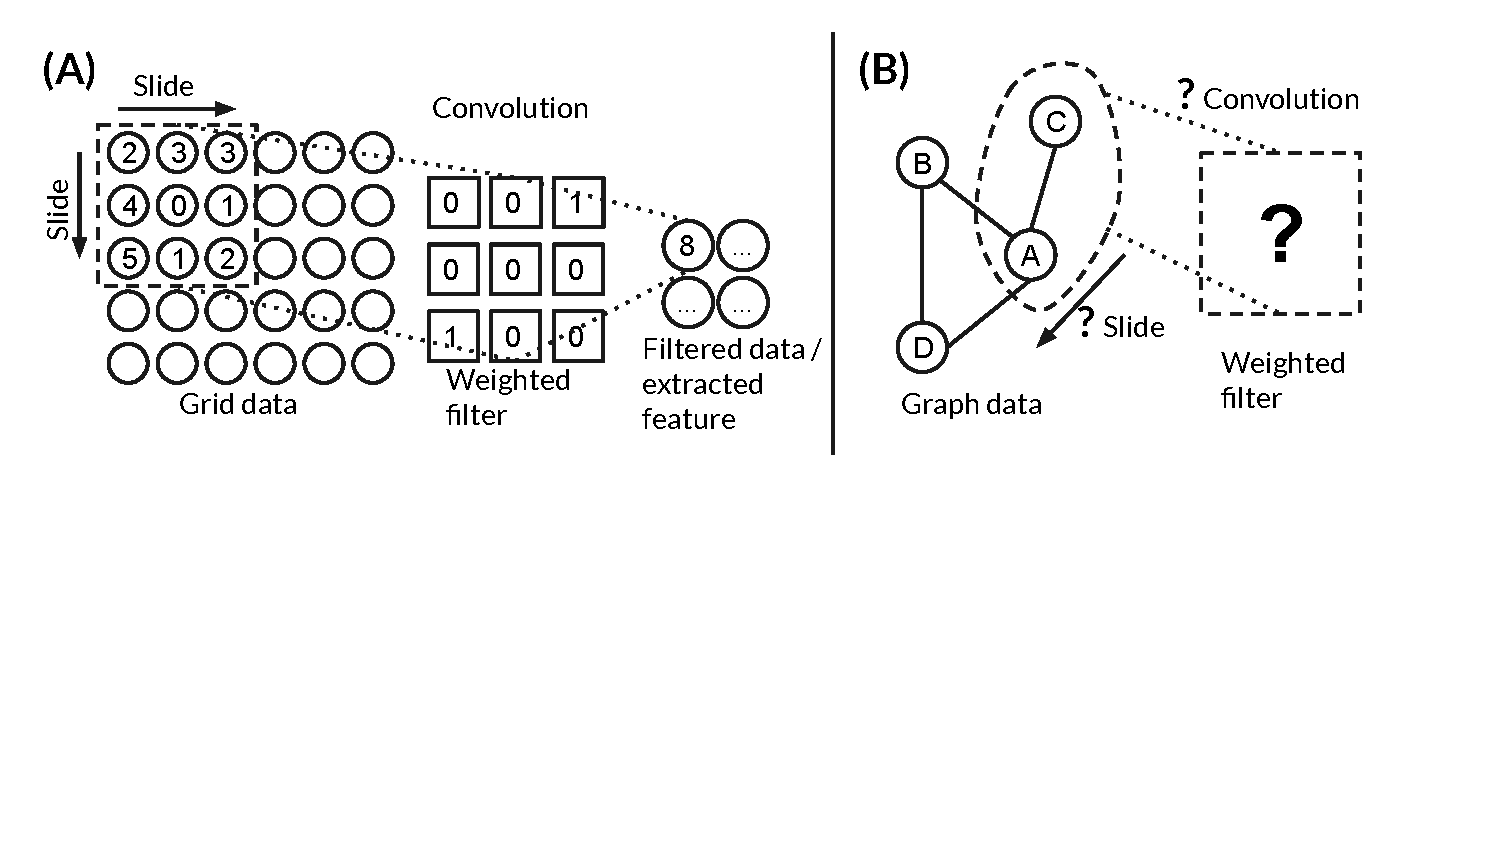
\includegraphics[width=0.49\textwidth]{./images/gridvsgraph.pdf}
 \caption{(A): Illustration of convolution on grid data such as image. (B): Natural operations such as translation and convolution on grid are non-trivial to define on graph data.}
 \label{fig:gridvsgraph}
\end{figure}

Deep neural networks, or deep learning, have revolutionized many domains like machine translation, computer vision, and natural language processing. They have proven to be highly effective in extracting complex and implicit features from the data. In many classical applications, the data is naturally represented as regular grids, such as images with their RGB pixel values. Techniques such as CNN~\cite{cnn0, cnn1, cnn2} are effective in capturing the local and shift-invariant information within an image. 

However, not all data has a simple grid or sequence shape; many data are naturally represented as graphs, while many other data can also be transformed into graphs~\cite{Xu2017}. Examples of graph data range from social and citation network~\cite{social, citation}, protein-protein interaction~\cite{ppi}, to point clouds~\cite{pointcloud}. Unfortunately, applying classical deep learning methods on graph data is not trivial, as graph data can have a rather irregular topology, and each node may have a different number of neighbors. There may not be ordering among the neighbors. Furthermore, the neighbors could be very distinct from each other, and there can also be information associated with the edges. These characteristics would make deep learning primitives such as convolution hard to define. As Figure~\ref{fig:gridvsgraph} presents, natural operations such as translation and convolution on a grid are not trivial to define for graph data.

Apart from the structural complexity, another distinctive characteristic of graphs is the absence of the i.i.d. assumption. In a classical machine learning setting, data points are usually assumed to be independently sampled from their actual distribution. However, data embedded in a graph as nodes are often explicitly connected, and these data are inherently non-i.i.d. This has complex implications when it comes to sub-sampling of graph data.

As such, there have been two directions to bring deep learning to graph data. The first route is by converting the graph data into the regular form to utilize existing deep learning methods; a prominent example is ~\cite{deepwalk}. The second route is developing new deep learning techniques or repurposing old techniques to work on graph data; these newly proposed techniques are known as Graph Neural Networks (GNN). This field has gained lots of attention recently and is the main topic of this paper.

Past efforts on GNNs can be roughly categorized into three divisions: the recurrent GNNs, spatial-based convolutional GNNs, and spectral-based convolutional GNNs~\cite{compsurvey}. The recurrent GNN and spatial-based convolutional GNN share very much in common, and they both explicitly leverage the structure and spatial localities of graphs. Hence, in some literature, they are also called spatial methods, while spectral-based convolutional GNNs are called spectral methods. Unlike spatial methods derived from deep learning research, spectral methods have a rather different lineage as they rise from the graph signal processing community. We will dive into the details later.
%
%GNNs have been used for various tasks, from local feature learning of node/edge embedding to global feature learning of graph embedding. They also have applications ranging from node classification, edge prediction, to generative tasks. These techniques have been used in various domains such as drug discovery~\cite{drugdis}, transportation research~\cite{trans}, particle physics~\cite{hep}, and many more domains~\cite{ss}

GNN research has not been solely focused on improving the accuracy performance of benchmark datasets. Lots of works focus on the system issues such as memory footprint and scalability~\cite{graphsage, fastgcn}. Apart from the algorithmic research and various techniques to bring down the computational cost, GNNs have also received attention from the system community. Just as the classical deep learning techniques need to be repurposed for GNNs, the underlying systems used for training/inference also need to change. The majority of the deep learning systems~\cite{tf, torch} had very little design consideration for graph data. As a result, their interfaces are unnatural for programming GNNs~\cite{dgl}, and their runtime performance is not optimal. 

Recently a new branch of system research has emerged: GNN systems~\cite{dgl}. These systems mainly focus on GNN model training and inference and optimize the execution to save time and avoid OOM errors. They are specifically tailored for graph data and GNN workloads, and they often offer orders of magnitude acceleration~\cite{dgl, pyg} over the classical deep learning systems.

Many surveys on GNNs exist~\cite{compsurvey, yannsurvey, zhousurvey} in the literature. However, none of them emphasizes the system issues and includes the newest advances in the GNN system domain. This paper is a short survey of GNN focusing on research related to the system issues of GNN. In addition to the algorithmic advancements, this paper will also go over some of the state-of-arts of GNN systems and provide potential future research directions. 

This paper is organized as follows: Section~\ref{sec:background} goes over some necessary backgrounds. Section~\ref{sec:gnn} covers various GNN architectures and the system issues and trade-offs associated with them. Section~\ref{sec:gnnsys} briefly introduces the emerging research field of GNN systems. Finally, Section~\ref{sec:conclusion} concludes this survey and discusses future research directions. 

%----------------------------------------------


\vspace{-2mm}
\section{Background and Preliminaries}
\label{sec:background}
\subsection{Deep Neural Networks}
Deep neural networks, or deep learning, have revolutionized many domains. To summarize its capability: one writes a set of simple goals (loss functions). Then, the program can automatically learn a way to represent the data and generate predictions for new data. Some prominent examples include CNNs~\cite{cnn2} and RNNs~\cite{rnn}. 

Recently other architectures such as Generative Adversarial Networks (GANs)~\cite{gan} and pure attention mechanism-based methods such as Transformers~\cite{transformer} have also greatly shaped the landscape. 

However, these techniques were majorly developed for regular-shaped data, such as tabular data, images, and time series. Naively applying deep learning to graph data is not viable. The model now needs to consider the underlying topology of the graph and must be capable of following the data relationship defined in the graph; the i.i.d. assumption commonly found in a lot of datasets may not hold for graph data. Therefore, graph data requires special treatment, and the DNN techniques usually need to be tweaked before applying to graph data.
%\subsection{Graph Analytics and Tasks}
%Graph analytics is a topic that has much longer history than GNNs. There have been abundant research and attempts to reason about graph data and extract valuable information from them. GNNs are among the newest additions to the arsenal of graph analytics and they have gained lots of attention. GNN, as  
%Node classification. Edge prediction. Graph embedding.
%
%\subsection{History of Graph Neural Networks}
%Prior to GNNs, there have been abundant research on graph analytics. However, the commonly acknowledged first published work on GNN was~\cite{gnn0}. This work purposed the first Recurrent GNN to better distinguish


\subsection{Machine Learning Systems for Efficient Model Training and Inference}
%The success of DNNs does not solely come from algorithmic advancements but is a combination of revolutions in computational hardwares~\cite{cuda}, availability of unprecedented large datasets (Big Data)~\cite{imagenet, coco}, and efficient and scalable systems designed for these novel workloads~\cite{tf, spark}. 
Because of the booming of DNN and their massive adoption across academia and industry, the demand for reliable, easy-to-use, and efficient software also skyrocketed~\cite{tf, torch, spark}. There are many aspects of the machine learning life cycle, from data sourcing, cleaning to model training and inference. Among these topics, model training and inference are arguably among the ones that face the most scalability and efficiency challenges; the complexity of the models and the amount of data has been rapidly growing up~\cite{gpt-3, toi}. It is vital for the model training and inference systems to keep up with the pace to enable such workloads at scale.  Again, due to the unique nature of graphs and GNNs, existing systems need to be tweaked and specialized for GNN workloads.

\subsection{Notations and Definitions}
We now summarize the set of notations and definitions used throughout the paper. Table~\ref{tab:notation} presents all the notations. We now give the definitions of several concepts. 
\begin{enumerate}
\item \textbf{Graph.} A graph $G(V, E)$ is defined as a collection of nodes $V$ and edges $E$ connecting the nodes. The graph can be directed or undirected, cyclic or acyclic. 
\item \textbf{Node and edge features.} Each node $v \in V$ can have a $D_v$-dimensional node feature vector $\mathbf{x}_v \in \mathbb{R}^{D_v}$. Similarly, each edge $e \in E$ can also have a $D_e$-dimensional edge feature $\mathbf{x}_e \in \mathbb{R}^{D_n}$. Stack these features as column-vectors to form matrix, we have matrix $\mathbf{X}_n \in \mathbb{R}^{D_v \times |V| }$ and $\mathbf{X}_e \in \mathbb{R}^{D_e \times |E|}$.
\item \textbf{Weights and model parameters.} Throughout the paper, the learnable weights of neural networks are typically denoted as $w$ (scalar), $\mathbf{w}$ (vector), or $\mathbf{W}$ (matrix). When it comes to weight matrices composed of weight vectors, they are usually row-based, in contrast to feature vectors and matrices. 
\item \textbf{Node neighbors.} Given a node $v$, the function $\mathcal {N}$ returns the set of all 1-hop neighbors of $v$, including the node itself. Similarly, define $\hat {\mathcal {N}}$ to be the function that returns all neighbors of a node, excluding itself. This includes both the nodes with edges pointing to $v$, and nodes pointed by $v$.
\item \textbf{Node embeddings and hidden states.} Node embeddings are representations of nodes in a Euclidean space through a usually learned mapping. They contain information about the node. In this paper, we use hidden states and node embeddings interchangeably. We use $\mathbf{h_v}$ throughout the paper to denote the node embeddings. The dimensionality $D_h$ is determined by the graph neural network and is usually a hyperparameter.
\item \textbf{Graph Laplacian.} Graph Laplacian is a matrix representation of the graph. It is very important in spectral graph theory and spectral-based convolutional GNNs, please refer to Section~\ref{sec:spectral} for details.
\end{enumerate}





\section{Background and Preliminaries}
\label{sec:background}
We start with some background on key technical concepts and notation needed for the rest of this paper.
\subsection{Deep Learning}
Deep learning (DL) refers to a technique for approximating patterns within data by applying gradient descent to optimize the parameters of a directed graph of operators. In this paper, we refer to the DL model graph as a \textit{model}, or a \textit{neural computational graph}. Feedforward networks are a particular type of computational graph wherein inputs are continuously fed forward through a chain of operators, each of which is known as a layer. Most large-scale model architectures fall under this class.

Common DL operators include \textit{matrix multiplies}, \textit{differentiable activation functions}, and \textit{embedding table lookups} (functionally equivalent to matrix multiplies with one-hot vectors). The first two are used for directly transforming data inputs while the latter is used for associating some personalized vector with a categorical input (e.g. translating an application user into a vector). A DL model might use all of these operators together in a complex structure, typically known as a deep neural network (DNN).

The \textit{training} of a model involves an optimization procedure called stochastic gradient descent (SGD). It samples \textit{mini-batches} of data from the training dataset, then runs a \textit{forward} pass through the model graph. The forward pass transforms the input data features into an output target, then calculates a \textit{loss} value, or error, relative to some ground truth \textit{label}. This loss value is used to run a \textit{backward} pass, also known as backpropagation. Backpropagation refers to the process of repeatedly applying the chain rule to calculate updates for each model parameter that will minimize the output loss. Note that in order for this chain process to work, intermediate outputs, also known as \textit{activations}, between operators \textit{must be saved}. \textit{Inference} applications, wherein the model parameters is frozen deployed for prediction, can discard intermediate outputs when transforming inputs, but training has to save the intermediates (which can bloat memory costs).

A full pass of minibatch samples through the entire dataset is called an \textit{epoch}. Training a model typically requires many epochs of SGD. Popular DL tools implement many variants of SGD (e.g., Adam, AdaGrad, RMSProp, etc.), known as \textit{optimizers} but their data access patterns are identical. Some optimizers maintain their own parameters and state which are updated during execution.

The size of a DL model can be measured through the number of parameters and/or its memory footprint. The memory footprint of a model is generally correlated with the number of parameters. In order to compute a full minibatch-pass, intermediate data must be materialized between layers, and gradients will also need to be held in memory as they are chained backwards during backpropagation. As such, an upper bound of model memory footprint can be made based on the sum of its parameters' memory costs, its intermediates' memory costs, and its gradients' memory costs. This upper bound is generally a high overestimate, since most training frameworks will automatically discard intermediates and gradients as soon as they are no longer needed.

\subsection{Deep Learning Accelerators}
Matrix multiplies are typically the most common and computationally intensive operators within DL model graphs. Other operators exist (e.g. activation functions, embedding table lookups) but these are generally less computationally intense. The general matrix multiply operation, or GEMM, is a well studied target for parallelization~\cite{blislab2016}. As such, using hardware that can exploit this opportunity effectively is a common practice among DL model developers.

\textbf{GPUs} offer stronger parallelization capabilities versus CPUs for simple operations such as the GEMM. In particular, Nvidia GPUs support the cuDNN library~\cite{cudnn}, which implements low-level DL operators tuned for parallelization on GPU threads. However, GPUs must operate on data stored within on-accelerator memory, which is far more limited than standard system memory (DRAM). A state-of-the-art consumer GPU typically has less than 40GB of on-device memory, while DRAM capacity on a training machine might easily exceed 512GB. 

\textbf{TPUs}, or tensor processing units, are a new type of accelerator developed by Google specifically for DL. TPU cores are organized to support parallelism in GEMM operations and experimental evaluations show that it can achieve up to 10X faster performance than GPUs on some model architectures~\cite{tpubenchmark2019}. Unfortunately, TPU access is still very limited --- practitioners can only use one through Google's Cloud Platform. As such, this survey will primarily focus on systems targeting GPU execution.

\subsection{Parallelization Techniques}\label{sec:parallelization}
A variety of techniques exist for parallelizing DL training. Each offers different advantages or drawbacks, which tend to vary depending on the workload. Understanding the data access and communication patterns of each strategy is critical to evaluating them in the context of large-model training.

\textbf{Model parallelism} refers to the technique of partitioning, or \textit{sharding}, a neural architecture graph into subgraphs known, and assigning each subgraph, or \textit{model shard} to a different device. In a feedforward network, these shards might refer to groups of stacked layers.

\begin{figure}[th!]
\centering
	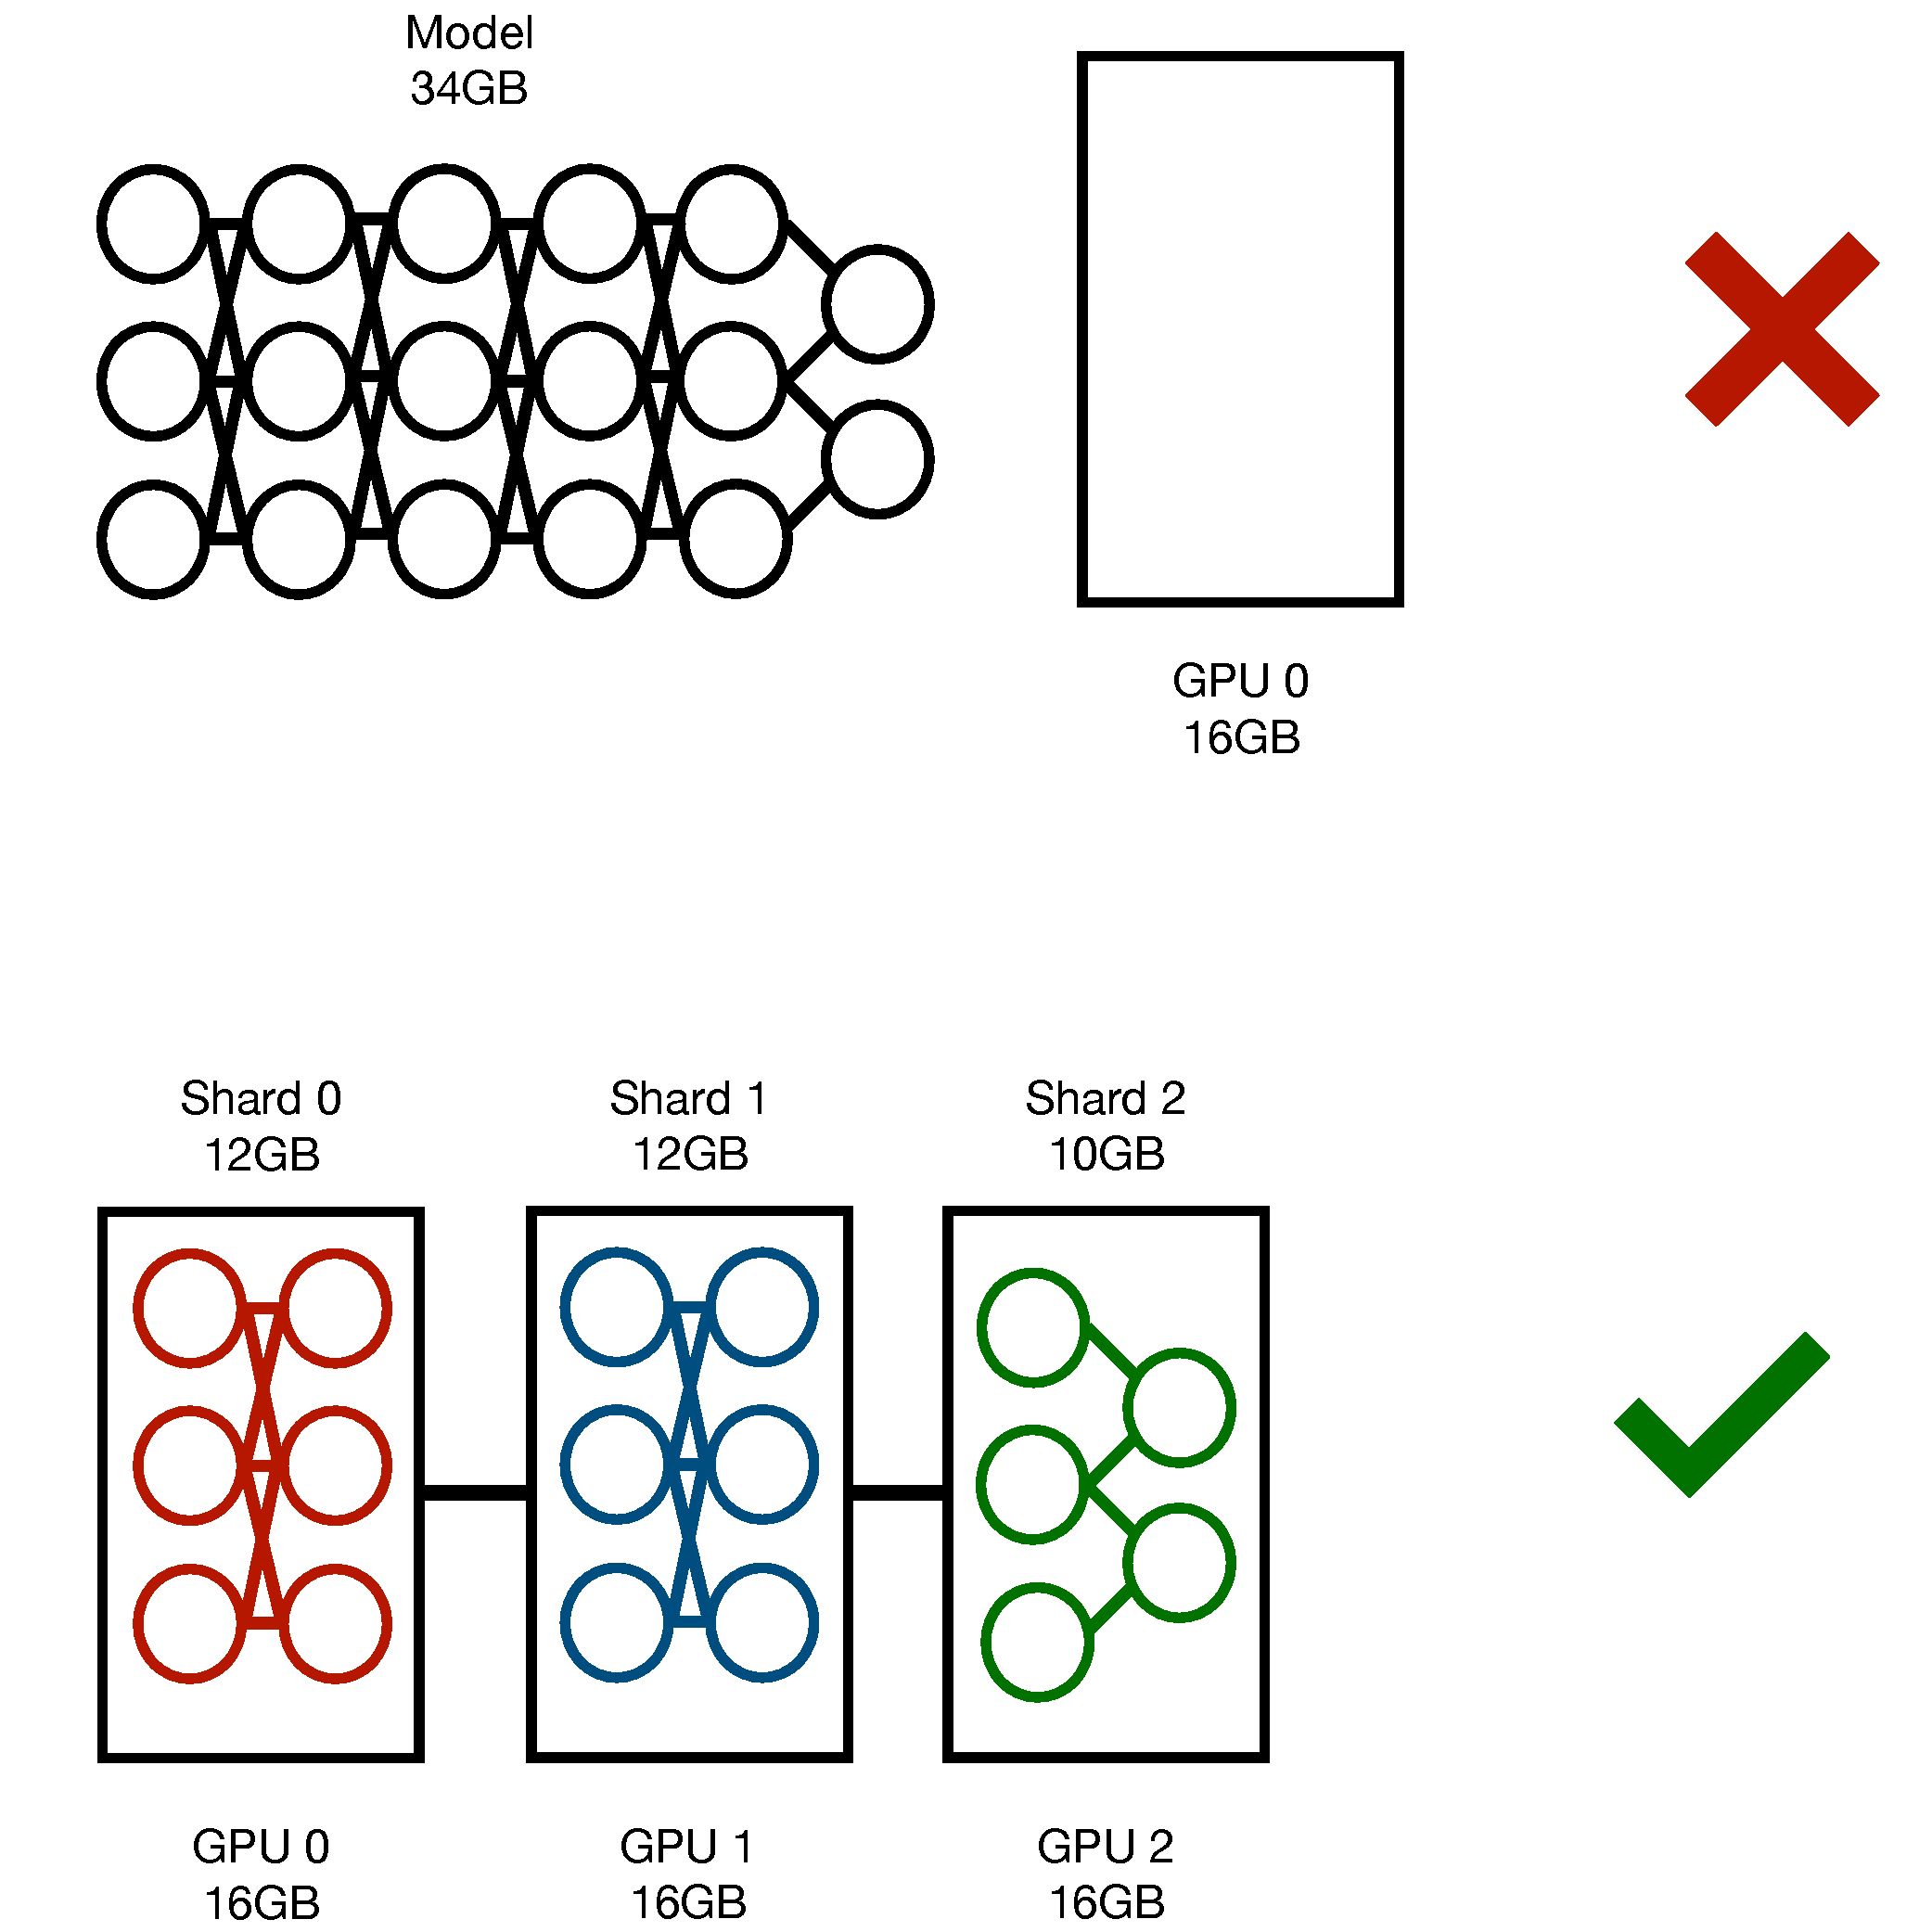
\includegraphics[keepaspectratio=true, width=0.9\linewidth]{images/model_parallelism_basic}
	\caption{An illustration of how a large feedforward network that does not fit into a single GPU could be model-parallelized over three GPUs to enable execution. Note that execution has not been sped up --- there is no parallel execution, only partitioned memory demands.}
	\label{fig:model_parallel_feedforward}
\end{figure}


The speedup potential of model parallelism depends largely on the architecture and the sharding strategy. Sequential model parallelism on a feedforward network, of the sort illustrated in Figure~\ref{fig:model_parallel_feedforward} will offer no scope for parallel execution, instead inducing a dependency graph between accelerators. This sharding strategy is still popular, however, as it can distribute memory demands across multiple devices and is fairly simple to setup. Other operators, such as embedding tables, are more amenable to being sharded width-wise as illustrated in Figure~\ref{fig:embedding_table_parallel}. Width-wise sharding strategies, more generally known as \textit{tensor parallelism}, can execute layers in parallel across multiple devices, but typically need to be followed by an all-gather communication pattern to produce a full output.

\begin{figure*}[th!]
\centering
	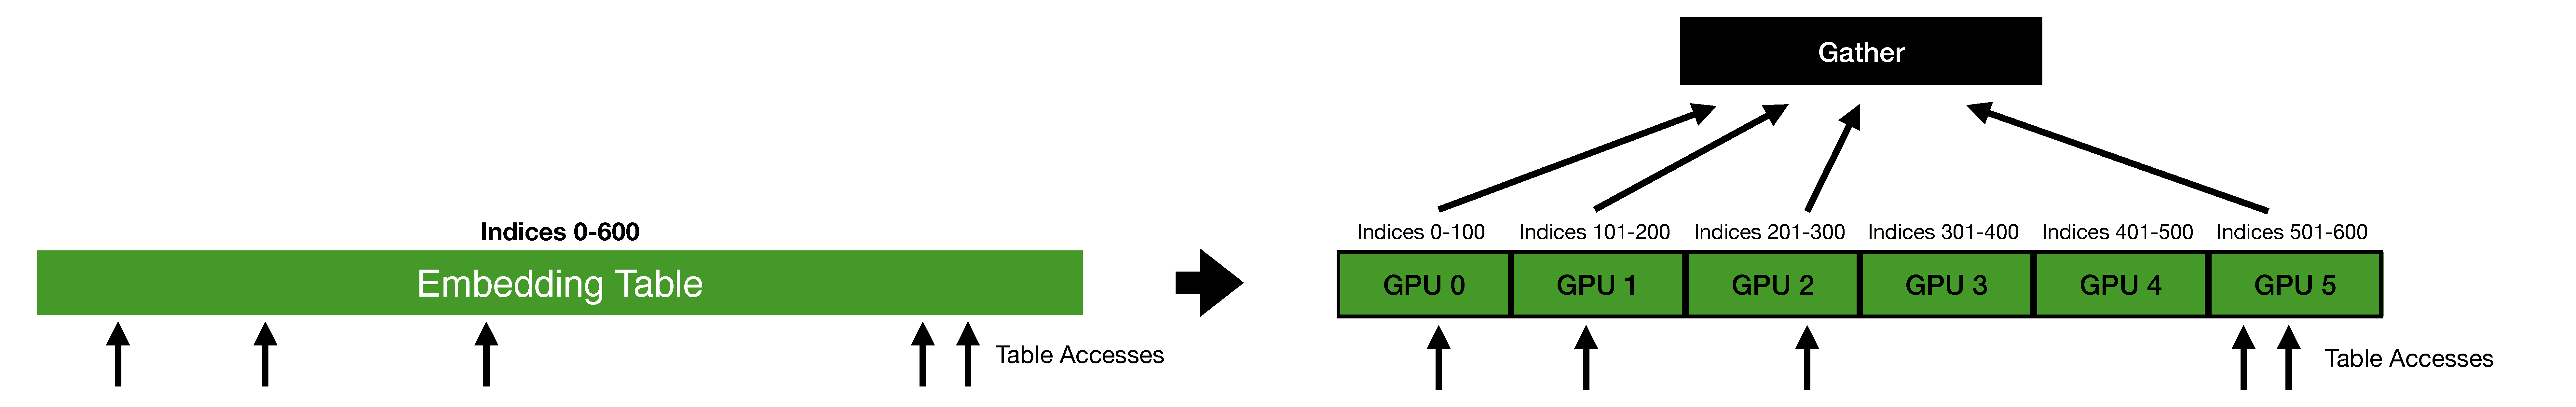
\includegraphics[keepaspectratio=true, width=0.9\linewidth]{images/embedding_table_parallel}
	\caption{An embedding table parallelized over 6 GPUs. Each GPU receives a different subset of the table's indices.}
	\label{fig:embedding_table_parallel}
\end{figure*}

Model parallelism of any sort introduces GPU-GPU communication. The latest Nvidia GPUs support ``NVLink'' interconnects --- high-speed GPU-GPU communication routes that offer as much as 900GB/s bandwidth --- which can help minimize overheads. NVLink is not always readily available, however, particularly when using cloud-provided machines that the user cannot customize easily. When NVLink is not supported, GPU-GPU communication runs over PCiE interconnects, which are much slower. The Tesla V100, generally considered a standard high-performance GPU for DL applications, supports a 16-lane PCiE 3.0 interconnect, at 16GB/s. 

To avoid having to transfer too much data over slow interconnects, model parallelism users generally aim to select a partitioning strategy that will minimize the size of activations that need to be transferred between shards, or else balance out computation to hide communication costs. Various sharding algorithms exist for this~\cite{flexflow2018,gpipe2019,lamp2020,mpanalysis2019,hydra2021,zero2019}.

\textbf{Data parallelism} is a common deep learning execution strategy that enables multiple mini-batches of data to be consumed in parallel. Data parallel execution techniques can be divided into two broad categories --- asynchronous data parallelism and synchronous data parallelism. 

The most well-known asynchronous technique is Parameter Server, wherein one core chief server holds a baseline set of parameters while distributed workers hold model replicas that train on different minibatches. The distributed workers occasionally send updates to the baseline server, which in turn will send out replacement parameters to the distributed workers to keep them updated. The workers can run out of sync with each other, as they only need to communicate/synchronize with the baseline server. Asynchronous techniques introduce many challenges, such as accuracy degradation versus single-worker training and irreproducible results due to variance in worker return times. For these reasons, asynchronous techniques are relatively uncommon in the modern DL training landscape. 

The most popular synchronous data parallel execution technique is Distributed Data Parallelism (DDP). DDP replicates a model and assigns copies to $m$ different accelerators. These replicas consume different minibatches of size $n$ in parallel and produce gradient updates for their local replica. These gradients are then aggregated across replicas to produce a global update, typically using an all-reduce communication pattern. This global update is then applied to every replica in parallel. This technique is mathematically equivalent to single GPU training with batch size $m \times n$. While this technique induces an all-reduce communication step, these overheads can generally be overlapped and hidden under model execution times.

\textbf{Hybrid parallelism} refers to strategies which \textit{combine} different parallelization strategies to achieve higher overall performance. For example, overlaying data parallelism on top of model parallelism could enable a user to achieve memory scalability across multiple devices along with the execution speedups of data parallelism. These strategies have tradeoffs that need to be factored into their design. In a simple overlay hybridization, model parallelism's multi-device requirements are multiplied by the replication requirements of data parallelism. A further overlay of task parallelism (e.g. in multi-model training) could add another multiplication factor into the equation. More complex hybridizations are covered in Section~\ref{sec:mlsys}.

\subsection{Model Modification}
Another approach is to actually reduce or alter the model itself to reduce its memory demands. Various techniques for \textit{compression} exist, some dynamic that readjust the architecture during training, and other static ones that reduce the model up front. Typically, compression induces an accuracy-size tradeoff, where higher compression factors reduce model learning capacity. This tradeoff can make this technique ill-suited to accuracy-critical applications, though well-managed and strategic compression can minimize the accuracy loss.

\textbf{Model distillation} attempts 


















\vspace{-2mm}
\section{Large Model Architectures}\label{sec:large_model}
To clarify the need for large model training systems and motivate their design, we describe various large model architectures and the unique challenges each presents. We can broadly classify the scale of model architectures under two categories --- depth-wise scaling and width-wise scaling. depth-wise scaling is most commonly needed for long, sequential chain architectures like Transformers. width-wise scaling is commonly used for very wide, easily parallelized operators (e.g. table lookups). A third setting, example scaling, describes the setting where the size of input samples drives the scaling challenge rather than the size of the model.This setting does not fall under the scope of ``large-model training'', so we do not discuss it in-depth in this paper.

\subsection{Deep Models \& Transformers}
Transformers, the most common example of very deep model architectures, have recently become very popular in a variety of domains. Benchmark tasks in natural language processing (NLP), computer vision (CV), and even tabular data analysis are now led by Transformer architectures. These models consist of stacked ``self-attention'' blocks, each of which consists of multiple dot product operations and matrix operations. Practitioners have found that increasing the depth of Transformers by stacking on more attention blocks generally improves accuracy~\cite{transformerStack}. As such, Transformers have motivated practitioners to explore increasingly deep model architectures. 

These models present a critical challenge for training. One of the first large Transformers was BERT-Large~\cite{bert2018}, using 345M parameters. The memory demands of training this model with a reasonable minibatch sample size on a GPU already required practitioners to use high-end GPUs. Since then, Transformers have only become deeper and deeper --- some recent ones have reached one trillion parameters, demanding space well beyond the memory capacity of \textit{any} GPU on the market. 

As such, techniques such as model parallelism are essentially necessary for large Transformer training, and deep model training in general. However, enabling parallel execution for very deep models can be challenging. The most natural sharding strategy for a deep sequence of layers is to partition the sequence into subsequences. But this approach forces the user to add GPUs without actually benefiting from any performance benefits ---- partitioning a sequence into subsequences does not offer any opportunities for parallel execution speedups. Consider a trillion parameter model that needs to use 1024 GPUs to even fit in memory. All of these GPUs are only being used to ``enable'' execution, and provide no performance benefits. In fact, the strategy would likely be slower than an equivalent in-memory training job due to the inter-GPU communication costs.

Some strategies for width-wise sharding exist, such as parallelizing operations in attention blocks across multiple GPUs. However, these approaches require more customization, add communication overheads, and require substantial effort on the part of the model designer to implement. As such, most systems for deep model training prefer to apply a generalized depth-wise sharding strategy that can be optimized for all deep model classes rather than targeting a single architecture at a time.

Despite the challenge of sequential dependencies, depthwise-sharding can introduce many opportunities as well. Techniques such as \textit{pipeline parallelism} and \textit{spilling} only work on depth-wise sharded models. We expand more on these techniques in Section~\ref{sec:mlsys}.

\subsection{Wide Models \& Embedding Tables}~\label{sec:embedding}
Wide models present a very different set of challenges from deep models. While it is easier to parallelize them in a performance effective manner (widthwise rather than depthwise), widthwise partitioning generally requires all-gather communication steps to aggregate parallelized partial outputs.

 \textit{Embedding tables} in recommender models are generally the most popular candidates for width-wise sharding. Embedding-based recommender models are used at most companies which gather entity-specific data (e.g. Meta, Netflix, TikTok) to create customized experiences. A standard approach is to create a table that maps user IDs to trainable vectors that can then be fed to some other DNN placed on top. However, for this to work on a multi-billion user platform such as Facebook, the corresponding table has to be very wide. A three billion index table with size 1024 trainable vectors filled with floats would require 12TB of memory. A real-world recommender might include \textit{multiple} such tables for different lookups (e.g. user table, business table, video catalog table), further increasing memory costs. 

Partitioning an embedding table is an easy task, given that table lookups are embarrassingly parallel --- a lookup on one index does not rely on other indices. As such, sharding a table into subtables assigned to different GPUs is a common strategy to distribute memory costs. Parallel execution across shards can easily be achieved by simply routing index lookup requests in a minibatch to the appropriate GPU. However, in order to re-aggregate the minibatch after the parallel table lookups (e.g. to feed to the top DNN), a potentially expensive all-gather communication step is necessary.

It is less common (but not unheard of) to apply width-wise sharding to other operators (e.g. very large matrix multiplies) can also be parallelized in a width-wise fashion. In general, embedding tables are the most memory-intensive single operators~\cite{dlrmscale2020}. Given that the primary use-case for width-wise sharding is embedding tables, optimizing for this case may seem overly specific. However, embedding tables and recommender models make up an outsized proportion of DL workloads --- Meta reports that 50\% of their DL training cycles are spent on embedding-table-based recommender models~\cite{dlrmscale2020}. As such, optimizing for the very wide model case is well worth it even if the applicability is more limited than optimizing for sequential deep model scalability.
\vspace{-2mm}
\section{Large Model Training Systems}\label{sec:mlsys}
Several systems have emerged to address the challenge of enabling efficient large-model training. We now describe the major classes of large-model training systems as well as key instances of each category. In general, most of these systems target a specific setting of large-model training (e.g. sequential deep models, wide models) as described in Section~\ref{sec:large_model}.

\subsection{Basic Techniques}
A few basic techniques such as rematerialization are often used as common building blocks for more advanced large-model training systems. In general, these techniques have minimal impact on organization and structure, making them amenable for integration with other approaches.

\subsubsection{Rematerialization}
Rematerialization, also known as gradient checkpointing, attempts to minimize the memory demands of \textit{backpropagation} specifically~\cite{checkpointing2000, checkpointing2016}. As explained in Section~\ref{sec:background}, backpropagation requires saving intermediate operator outputs for proper application of the chain rule for gradient computation. However, intermediate output tensors can demand a great deal of memory!  Some analyses~\cite{lowmemory2019} have shown that activations make up as much as 95\% of memory consumption for ResNet~\cite{resnet2015} and as much as 80\% of memory usage for some Transformers. Rematerialization trades compute for memory by initially discarding most of the activations except for a few \textit{checkpoints}, then \textit{recomputing} the discarded during backpropagation using the checkpoints. In this way, only the intermediates between checkpoints need to be stored in memory at any given point.

This approach does induce computational overhead --- the forward pass is effectively being run \textit{twice}. However, the operators in the forward pass are generally faster than the automatic differentiation procedure used in backpropagation, so the overhead is smaller than it might seem. Some gradient checkpointing systems claim to have only 30\% overheads for 6-7X memory savings~\cite{checkpointing2016}.

Checkpointing is critical to techniques such as \textit{pipeline parallelism} and \textit{shard alternator parallelism}.

\subsubsection{Accumulation}\label{sec:accum}
Accumulation targets the memory demands of batched \textit{gradients} in backpropagation~\cite{gpipe2019}. Section~\ref{sec:background} describes how stochastic gradient descent batches samples into minibatches that are fed through the model. In turn, we can consider the gradients that are produced for parameter updates to be the aggregation of the updates that would have been applied for each sample. Accumulation delays the application of these aggregated gradients, instead computing new minibatch-gradient-updates and accumulating them onto our aggregated gradient vectors. The new gradient is now the aggregated sum of \textit{2} minibatch updates, rather than 1. In this way, we can scale up our effective minibatch size and gradient impact without actually training a larger batch. We refer to the smaller, individual batches as \textit{microbatches}, and keep referring to the effective summed batch as the minibatch. 

Accumulation is essential to \textit{pipeline parallelism}, and is often used in conjunction with other techniques.

\subsubsection{Low Precision Representations}
Most training frameworks (e.g. TensorFlow, PyTorch)\red{Cite them} use single-precision float (32 bit) representations of gradients and parameters. Double-precision representations (64-bit) are relatively uncommon. One way to reduce the memory demands of training a model is to use \textit{half-precision} (16 bit) representations of data. Naturally, this induces an accuracy loss as values are being approximated. However, this approach can offer both speedups and memory savings. To try and balance this, \textit{automatic mixed precision}~\cite{amp2020} will automatically try and determine when data can be safely compressed to 16 bit without accuracy losses. AMP generally reports little-to-no accuracy losses while achieving as much as 5.5X speedups when training large models~\cite{amp2020}. Since AMP is directly modifying values at a very low-level, this technique is generally orthogonal to actual systems approaches for large-model training. 

\subsubsection{Sparse Representations}
In some cases, the vectors used in DL training are very sparse. As an example, embedding table lookups generally only involve a few indices of the table. The gradient vector applied to the table will only have non-zero values at the used indices, while the rest of the gradient will be zeroed out. Actually maintaining all of these zeroes in memory is unnecessary and wastes memory. Sparse representations attempt to compress these vectors down to their non-zero values while avoiding any information loss. The most simple approach, commonly used by default for embedding tables, is to represent a gradient as key-value pairs mapping indices to gradient values. An example is illustrated below.

\[ <0, 0, 0, 0, 0, 0, 4, 0> \rightarrow \{6: 4\} \]

This representation can easily be mapped back for application while discarding unnecessary zero values.

Some complications arise when combining sparse representations with operations that assume standard vector representations, such as all-reduce communication patterns. Some works~\cite{mlplatformmeetup2022} show how this can be resolved by more complex communication patterns or as-needed conversions back to standard representations. Sparse vector representations address a very specific problem, but are critical for efficient training of some operators such as wide embedding tables.

\subsection{Pipeline Parallelism} \red{add citations}
Pipeline parallelism targets the ``sequential deep model'' setting. It is a direct extension of the model parallel training paradigm described in Section~\ref{sec:background}. Model parallelism creates a staged-out sequence of shards, creating a natural ``pipe'' structure. Pipelining simply exploits this pipe structure by attempting to fill up the stages with operations, reducing the idling that sequential model parallelism suffers from. Consider the example of a pure feedforward network, like the one illustrated in Figure~\ref{fig:model_parallel_feedforward}. Each shard can be considered a stage of the pipe, such that a model partitioned three-ways over three GPUs is now a three-stage pipeline.

In CPU pipelining, we fill up the pipeline with various instructions being sent to the CPU\red{find citaition}. For DL pipelining, we fill up the pipeline with microbatches, like those used in gradient accumulation. In essence, pipeline parallelism is the combination of gradient accumulation and model parallelism. Independent microbatches are shuttled through the shard pipeline, then gradients for each microbatch are accumulated for each pipeline stage. Once the gradients for the full minibatch (combination of all microbatches) are all aggregated, they can be applied to the model.

Backpropagation presents a challenge for pipeline parallel training. As explained in Section~\ref{sec:background}, intermediate outputs must be available for backpropagation to occur. When combined with accumulation, however, this would require us to store a different intermediate output set for each microbatch, thus robbing us of any scalability advantage offered by accumulation. GPipe~\cite{gpipe2019}, one of the first pipeline parallel training systems, proposed combining accumulation with checkpointing to address this issue. Activations would only be stored at shard/pipe stage boundaries, with recomputation occurring as gradients shifted backwards through the pipe during backpropagation. The checkpointing approach is now standard in most, if not all, pipeline parallel training systems.

Another challenge is presented by the structure of the pipe. For pipelining to work, the shard pipe must be bidirectional. Input and activations flow forward during prediction, and gradients flow backward during backpropagation. This leads to a problem --- data within the pipe will ``collide'' on stages as it flows in both directions. As such, a pipeline flush occurs between prediction and backpropagation. The flush can severely hurt performance if not properly managed. Figure~\ref{fig:pipeline_parallel} illustrates a pipeline parallelized model. Note that all three accelerators are only active on steps 4 and 10 --- the rest of the time at least one accelerator is idle.

There have been many attempts to address this issue. GPipe~\cite{gpipe2019} suggested increasing microbatch counts while keeping accelerator counts constant, so the pipe could stay full for longer. This would not \textit{eliminate} the flush, but it would improve overall efficiency. However, this approach would demand more memory to store more checkpointed microbatch activations as well as larger input batches (potentially affecting convergence).

Another solution was proposed in the form of \textit{asynchronous pipelining}, which would reorder pipeline stages and backpropagation to eliminate the flush. Rather than running the stages for one microbatch in a sequence, they might run for one stage then be paused while a different microbatch runs a different stage. This ``decoupling''  of the order relaxes the problem into a more efficient one --- at the cost of affecting data consumption ordering and consumption. The 1F1B pattern runs one forward stage for every backward stage (on different microbatches) to maintain a perfect ratio and utilization. While asynchronous pipelining can perform well, it should be noted that it is not a general solution --- the accuracy losses are case-specific and can often be substantial. Applications where accuracy is critical and convergence behaviors must be replicable (e.g. model selection) are not a good fit for asynchronous pipelining.

\begin{figure*}[th!]
\centering
	
\includegraphics[keepaspectratio=true, width=\linewidth]{images/model_parallel_pipeline_parallel}
	\caption{An illustration of pipeline parallelism over three shards. The input minibatch is partitioned into \textit{microbatches} that are then shuttled through the pipe stages. Before backpropagation, the forward prediction pipe has to fully clear, leading to idling. All microbatches must be backpropagated prior to gradient application for mathematical equivalence, as explained in Section~\ref{sec:accum}. \red{Shrink Image to make text legible}}
	\label{fig:pipeline_parallel}
\end{figure*}

\subsection{Memory Offloading \& Spilling}\label{sec:spilling}
While model parallelism looks at execution over multiple GPUs to distribute memory demands, some systems attempt to make use of main system memory (DRAM) rather than horizontally scaling across more GPUs. The primary motivation for this approach is that while GPU memory is limited and expensive, DRAM is substantially cheaper and readily accessible.

Consider an AWS-provided p3.2xlarge node. It has a single V100 GPU with 16GB of on-device memory. A large DL model might not fit into the node's GPU memory, but in actuality the node has far more \textit{total} memory still available --- 61GB of DRAM plus the 16GB of GPU memory. DRAM (sometimes referred to as CPU memory in the ML systems literature~\footnote{We consider the term CPU memory is ambiguous, given that it could be interpreted to refer to registers or CPU caches. In this paper, we use the term DRAM to refer to main system memory, but it should be noted that other ML systems papers may use the phrase CPU memory to refer to the same concept.} is far cheaper and more available than GPU memory, and a standard cloud-provided multi-GPU machine might easily have hundreds of GBs of DRAM. 

If a model's memory demands can be spread across both DRAM and GPU memory, a large model could be trained without the need for model parallelism's multi-GPU costs. A on-demand AWS p3.2xlarge node offers 77GB aggregate memory at a rate of \$3.06 per hour. In order to have the same amount of GPU-only memory, a p3.16xlarge 8-GPU node would be necessary --- costing the user \textit{8X as much} at \$24.48 per hour.  Note that this is not an exact comparison --- the p3.16xlarge node actually has 128GB of memory rather than 77 due to how AWS allocates DRAM-GPU count ratios, and GPU memory does not perform in precisely the same way as DRAM. But the general point is clear --- for pure storage purposes, making use of DRAM is far more cost-effective than scaling up to more expensive higher-GPU-count machines. As such, offloading part of the memory demands of a model to DRAM rather than scaling across multiple GPUs can be an attractive option for cost-conscious users (e.g. small enterprises and researchers). 

Many initial works~\cite{tflms2019,meng2019,swapadvisor2021,vdnn2016,wang2018} treated offloading as a ``swapping'' problem --- deciding when to swap tensors off of GPU memory and onto DRAM. Most use graph analysis algorithms to determine where to ``inject'' a swap operation based on when an activation, gradient, or parameter might next be used in the execution graph. SwapAdvisor, the most advanced of these swapping systems, uses a parallelized genetic search algorithm to analyze where the swap operators should be placed for best performance. It was also one of the first systems to support offloading \textit{parameters} as well as activations, which is critical for training recent large model architectures which use billions of parameters.

These complex swapping procedures can be difficult to setup --- SwapAdvisor's search algorithm takes roughly an hour to complete. Moreover, they are difficult to extend to multi-GPU training, as there is no clear way to extend the swap-injected graph technique to cover multi-GPU parallelism.

Another approach was proposed with ZeRO-R~\cite{zero2019}, a system for offloading that sends activations and parameters to DRAM dynamically. This approach ``offloads when needed'', rather than planning offloads up front. The irregularity of the design can introduce issues such as memory fragmentation, but it adds a great deal of flexibility versus graph-based designs. A later version, ZeRO-Infinity~\cite{zero2021} extended this to offloading to NVMe/disk storage for further scalability.

Hydra~\cite{hydra2021} opts for an ``independent block'' strategy, dividing a model architecture into submodels (like model parallelism) that can then be spilled between DRAM and GPU memory freely. An analogy can be drawn to spilling in RDBMSs, where independent data chunks can be sent down to a lower level of memory. Unlike other spilling systems, Hydra's execution pattern is identical to model parallelism, and separates the execution of each model shard entirely. It still tries to overlap communication and computation, but ignores the complexities of fine-grained tensor offloading explored by other CPU-offloading techniques. This generalization makes it less-than-optimal for single-GPU execution, but makes it far more amenable to hybridization with multi-GPU parallelization techniques. We expand on this further in Section~\ref{sec:mt_parallel}.

L2L~\cite{l2l2020} uses a design similar to Hydra's but is more restricted in its sharding approach. It targets Transformer architectures specifically, and swaps across self-attention blocks with heuristics selected specifically for its target class of models. This allows it to perform very well on Transformer architectures, but prevents it from achieving the flexibility of Hydra or the dynamic generality of ZeRO-R.

Note that these techniques are generally used for distributing \textit{depth-wise} large model memory demands, as they all exploit some kind of sequential ordering in execution. A very wide operator (e.g. an embedding table) that cannot be serialized without substantial performance slowdowns, cannot easily be spilled across DRAM and GPU memory. The only option for hybrid-device execution on wide operators is to either serialize the parallel operator (index lookup in the table case) and rewrite the series of operations into a deep, rather than wide, model, or else to actually execute the wide operator on the CPU. 

Some systems combine offloading with mixed CPU-GPU computation. In general, it is preferable to run a model entirely using GPU or TPU compute, as most DL operators will run much faster on accelerators that support high degrees of parallelism. In the memory-limited case, however, it may become more practical to run some memory-intensive operations on the CPU using DRAM storage for operands rather than executing everything on the GPU.

ZeRO~\cite{zerooffload2021} proposed running parameter updates on the CPU while GPU execution is ongoing, specifically for the popular Adam optimizer~\cite{adam2014}. The Adam optimizer holds some state parameters (typically 32-bit) and needs to run on 32-bit parameters to avoid accuracy degradation. Unfortunately, this prevents users from exploiting 16-bit representations for reduced memory demands. The ZeRO version of the Adam optimizer maintains 32-bit versions of the parameters on DRAM and low-precision 16-bit versions on the GPU to consume less memory. During execution, the system spills gradients and optimizer state onto DRAM, then runs parameter updates on the 32-bit parameters using \textit{CPU processing}. The updates are propagated back to the 16-bit parameters in a secondary step that overlaps CPU-GPU communication with GPU computation. 

Mixed-CPU-GPU compute is also common for very large recommender models. As explained Section~\ref{sec:embedding}, embedding tables are very wide memory-intensive operators which generally feed into some smaller DNN for further processing. Without any optimization, the sheer scale of the embedding table would force CPU-only execution~\cite{dlrmscale2020}. Alternatively, a user could place the embedding table on the CPU while the DNN sits in GPU memory and enjoys the benefits of GPU acceleration. Some works such as Hotline~\cite{hotline2020} try and pipeline data through the model, from the CPU-based embedding table into the GPU-accelerated DNN. They demonstrate that this mixed compute approach can be even faster than width-wise multi-GPU model parallelism, as it eliminates the need for the all-to-all communication step described in Section~\ref{sec:embedding}.

\subsection{Hybrid Parallelism}
The basic parallelization techniques described in Section~\ref{sec:parallelization} can be combined in different ways. Various systems have attempted to combine the benefits of the various ``basic'' parallel execution approaches (e.g. data parallelism, model parallelism) to offer users higher performance and scalability. Hybrid parallelism techniques can be classified into two broad categories --- ``true'' hybrids that integrate parallelization techniques from the ground up, and top-down hybrids that select between different strategies at different stages of execution. 

\subsubsection{Ground-Up Hybrids}\label{sec:mt_parallel}
Traditionally, combining model parallelism with other techniques from the ground up has been a challenging task. Model parallelism drives up the GPU requirements of standard execution, which can make combinations with replication-based or multi-instance techniques for parallelism (e.g. data parallelism, task parallelism) impractical as they scale up model parallelism's device requirements further still. To address this problem, Hydra~\cite{hydra2021} proposed using the spilling technique outlined in Section~\ref{sec:spilling}.

\subsubsection{Fully-Sharded Data Parallelism}\label{sec:fsdp}

\subsubsection{Strategy Finding}

\subsubsection{Model-Data Parallelism for Recommender Models}

\section{Conclusion and Discussion}
\label{sec:conclusion}
In this paper, we surveyed GNN research, ranging from pioneering works to milestone papers. GNN research is gaining enormous attention, and scalability and efficiency have been one of the major topics.
We now discuss the potential research directions on the scalability and efficiency of GNNs.

On the algorithmic research of GNNs. Sampling has proven to be a very effective way of increase GNN efficiency. However, graph sampling is non-trivial because of the non-i.i.d. nature of graph data. Moreover, ignoring the interconnections may lead to degraded accuracy performance. Therefore, sophisticated sampling that considers the connections while still offering a boost in efficiency and scalability is a very important problem. Similarly, graph coarsening, which distills the original graph to be smaller subgraphs, can also significantly improve efficiency.

On the GNN system research. One natural direction for GNN system research is to scale out, i.e., distributed processing, which is receiving attention. On the other hand, they face even more problems like graph partitioning and load balancing. As mentioned before, the graph data is non-i.i.d., thus both sampling and partitioning are difficult to do. Graph partitioning for GNN itself is already a hard problem, let alone considering load-balancing simultaneously. The other important direction is compilers that can generate fused kernels for GNN operations, given a set of arbitrary user-defined functions. Such innovation would be especially useful for algebraic approaches. Meanwhile, existing general-purpose graph analytics systems may have more to offer, especially on the front of scalability and when the system needs to operate on huge graphs.


%\begin{table}[t]
\centering
\caption{Notations used in this paper.}
\scalebox{0.90}{
\begin{tabular}{@{}ll@{}}
\toprule
Notation & Description \\ \midrule
$G(V, E)$     & A graph $G$ with nodes set $V$ and edges set $E$        \\
$v, e$     & Node and edge        \\
$\mathbf{x}_v, \mathbf{x}_e$     & Node and edge features of $v$ and $e$, respectively      \\ 
$\mathbf{X}_V, \mathbf{X}_E$     & Matrices where node/edge features stacked up as columns      \\ 
$\mathbf{h}_v$     & The hidden states/node embedding of $v$      \\ 
$\mathbf{H}_V$     & The column-stacked matrix of all $\mathbf{h}_v$     \\ 
$D_v, D_e, D_h$     & Dimension of node and edge features, and hidden states      \\ 
$w, \mathbf{w}, \mathbf{W}$     & Scalar weight, weight vector, and weight matrix      \\ 
$\mathcal{N}(v)$    &  Function that returns the neighbors of $v$, including $v$      \\ 
$\hat {\mathcal{N}}(v)$    &  Same as above, excluding $v$      \\ 
$\mathbf{A}$ &  The adjacency matrix     \\ 
$\mathbf{D}$ &  The degree matrix     \\ 
$\mathbf{L}$ &  The graph Laplacian     \\ 
\bottomrule
\end{tabular}
}
\label{tab:notation}
\end{table}

\begin{figure*}[h]
 \centering
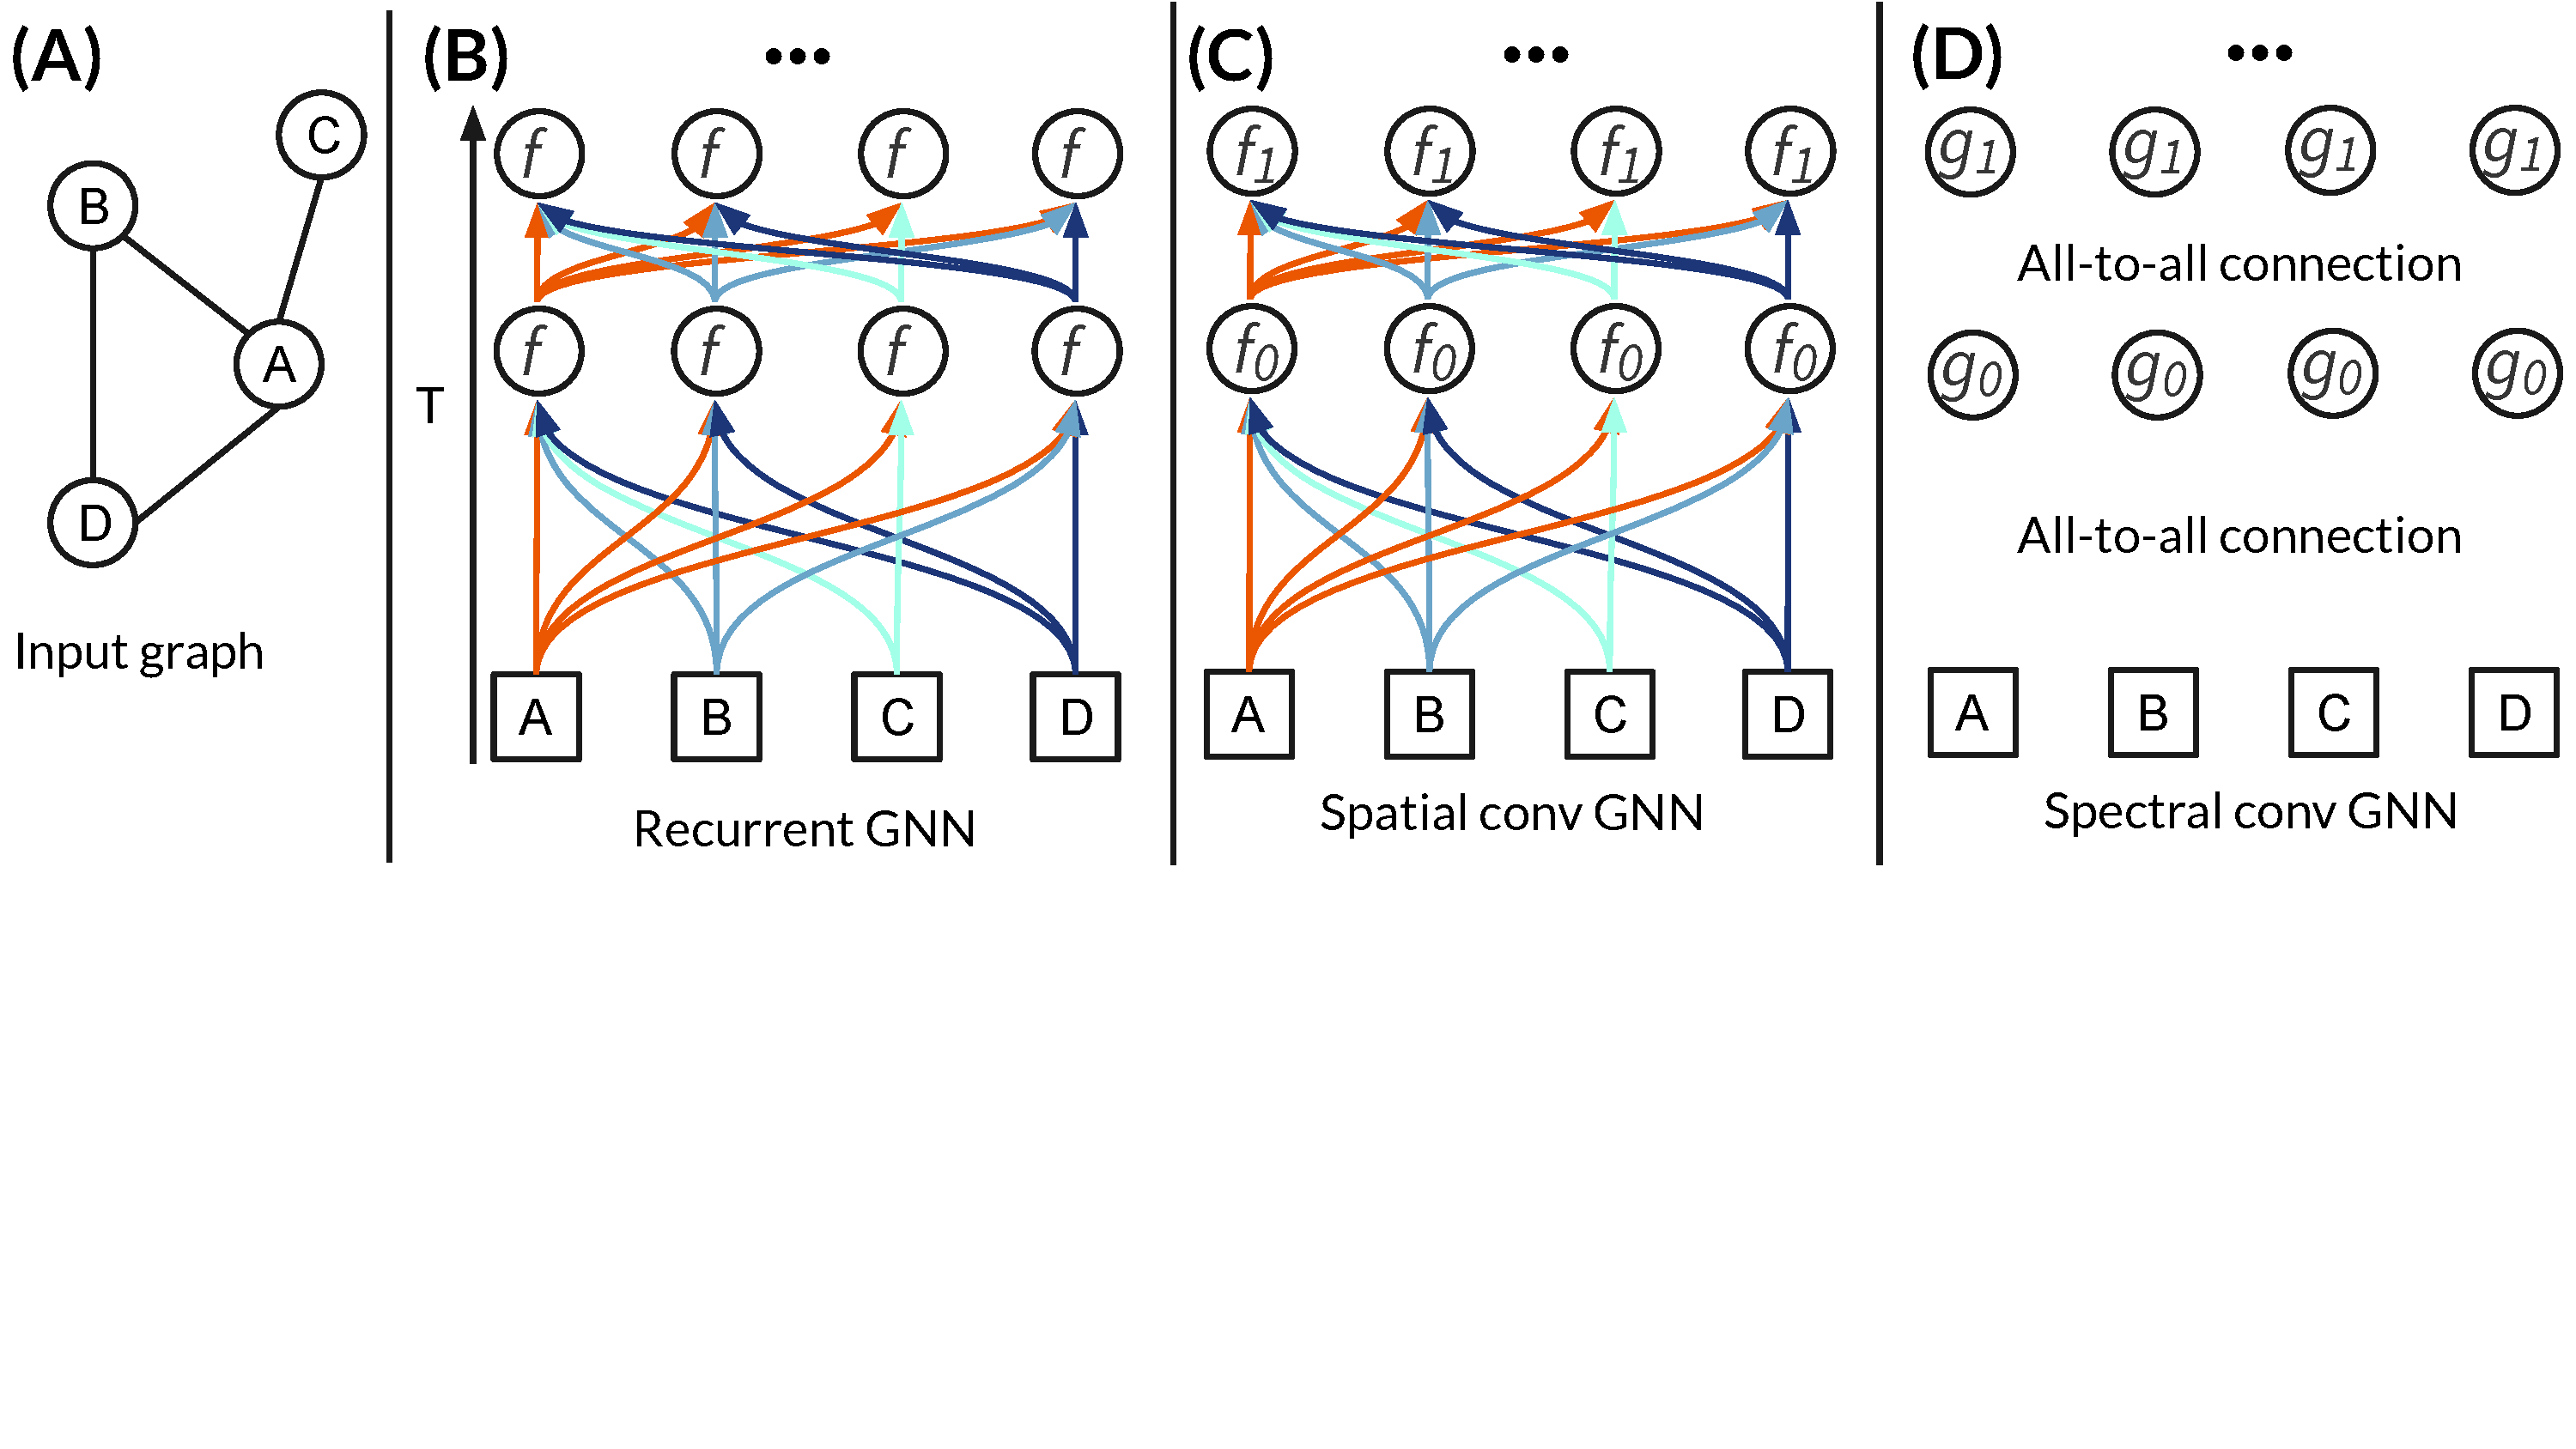
\includegraphics[width=0.75\textwidth]{./images/conceptual.pdf}
 \caption{Conceptual comparison of GNN architectures. (A): Input graph. (B): Recurrent GNN. Same function is applied recursively through time. (C): Spatial-based convolution. Different filters are applied in different layers. (D): Spectral-based convolution. Filters operate on the entire graph, unlike locally in (B) and (C).}
 \label{fig:conceptual}
\end{figure*}

\vspace{-2mm}
\section{Graph Neural Networks}\label{sec:gnn}
We now go over some representative graph neural network architectures. Roughly speaking, there have been three major branches of GNN: the recurrent GNN, the spatial-based convolutional GNN, and the spectral-based convolutional GNN. The first two types exploit spatial locality information in a graph. Therefore they are also collectively called the spatial method. In contrast, the latter one is called the spectral method, as it conducts graph convolution through a point-wise product in the graph Fourier space, based on the convolutional theorem. Such Fourier transformation requires global information of the graph. Figure~\ref{fig:conceptual} shows a conceptual comparison between these methods.

Beyond spatial and spectral methods, there also exist other GNN architectures such as graph generative adversarial networks (Graph Autoencoders and GANs)~\cite{gae, ggan} and spatial-temporal GNNs~\cite{gaan, stgnn}. However, there are overlaps between them and spatial/spectral methods, and many of these architectures rely on primitives such as graph convolution. Due to space limits, this paper will focus on the spatial and spectral methods, as they are deemed more fundamental.


\subsection{Recurrent GNNs}
Recurrent GNNs are analogous to the Recurrent Neural Networks (RNNs) in the sense that they both contain a recursive neural network layer and apply the same set of parameters to different parts of the input data. Many of the first published works of GNN~\cite{gnn0} falls into this category, and there have been numerous subsequent works~\cite{gesn, ggnn, sse}. In the original paper, the architecture is simply named GNN, and in this survey, we will call it GNN-0 to differ from other GNNs.
\subsubsection{The Graph Neural Network Model (GNN-0)}\hfill \\
GNN-0~\cite{gnn0} is commonly known as one of the first works on graph neural networks. It calculates the hidden states of each node through a message passing/diffusion model, in which the hidden states of nodes are treated as information that can freely flow within the graph. Then each node's hidden state would finally reach equilibrium. Mathematically, the update rule for node $v$ at step $t$ can be written as:
\begin{gather}
\mathbf{h}_v ^t = \sum_{u \in \hat {\mathcal {N}}(v)} f(\mathbf{x_v}, \mathbf{x_u}, \mathbf{x_e}, \mathbf{h}_u^{t-1}),
\end{gather}
where $f$ is a learnable function and implemented using a fully connected neural network. For simplicity, define a single variate function to be:
\begin{gather}
f_w(z) = \sum_{u \in \hat {\mathcal {N}}(v)} f(\mathbf{x_v}, \mathbf{x_u}, \mathbf{x_e}, z)
\end{gather}
The graph's hidden states/node embeddings are said to be in equilibrium if:
\begin{gather}
\mathbf{h}_v ^t = f_w(\mathbf{h}_v ^{t-1}),
\end{gather}
which indicates that the neural network does not further alter the hidden states of the node and that $\mathbf{h}_v ^t$ is the fixed point of the function $f_w$. Additionally, another fully connected layer, denoted as function $g$, is added at the end of propagation to generate predictions based on the hidden states. The loss is then calculated based on the predictions and can be backpropagated to both $g$ and $f_w$ during training. The choice of using a multilayered neural network to implement $f$ and $g$ is convenient. However, this fixed point does not always uniquely exist unless if the function $f_w$ is a contraction map (Banach fixed-point theorem), a characteristic that a plain fully connected neural network does not possess. Therefore, to guarantee the uniqueness and existence of the fixed point, a correction term needs to be added to the loss function. This correction term would put constraints on the Jacobian of the neural network and consequently force it to be a contraction mapping.

GNN-0 resembles the form of a recurrent neural network, except it has a graph shape, while RNNs are list-like. Recurrent GNN has very similar characteristics with RNNs and shares the same training paradigm. A common practice is to unroll the GNN-0 in time, just like RNN, and Figure~\ref{fig:conceptual} (B) shows the unrolled network. The structure of the graph determines the connections between each layer. To train such a GNN model, common methods such as backpropagation through time (BPTT) can be adopted. However, the BPTT algorithm requires storing all the intermediate hidden states during the forward propagation, which drastically increases the memory footprint as the algorithm scales linearly with the number of layers. 

To overcome the memory issue of BPTT, GNN-0 adopts Recurrent Back-propagation (RBP), also known as the Almeida-Pineda algorithm~\cite{almeida, pineda}. RBP is a method for recurrent neural network training, and it is applicable when the hidden states of the recurrent neural network converge to a fixed point, which GNN-0 exactly does. RBP has a significant memory footprint reduction compared to BPTT as it stores only the hidden states of the last layer of recursion, meaning constant space complexity on a given graph and independent of the recursion depth. RBP works as follows iteratively: it first conducts a recursive forward propagation until the network reaches equilibrium. Then instead of unrolling the network in time, it conducts a recursive backpropagation until the gradients also become stable. It then applies the gradients and repeats for the next iteration.

Even with RBP to control the memory footprint, GNN-0 still faces various issues: as a recurrent neural network, it has the same problems RNNs face. It also conducts gradient descent (GD) that needs the whole graph and all hidden states for each iteration, while the de-facto deep learning training framework is stochastic gradient descent (SGD). Existing systems are mostly optimized for SGD training~\cite{cerebro, tf, torch, horovod}. There are attempts to apply SGD to recurrent GNN~\cite{sse}, but it is unknown if it still theoretically guarantees convergence to a fixed point. Furthermore, the constraint of contraction map GNN-0 was pointed out that it may hinder the expressive power of the neural network and may cause dropped performance for long-range dependencies~\cite{ggnn}.

\subsubsection{Gated Graph Neural Network (GG-NN)}\hfill \\
GG-NN~\cite{ggnn} is a follow-up work to GNN-0. It applies a gated recurrent unit (GRU) to construct the update rule of hidden states. Because of this, GG-NN does not guarantee a fixed point anymore and there is no need for the neural network to be contraction mapping. For the same reason, GG-NN requires an initialization the node embeddings, which are chosen to be the node features. GNN-0 does not need such initialization since the exponentially quick convergence is guranteed. The update rule of GG-NN can be written as:
\begin{gather}
\mathbf{h}_v ^0 = \mathbf{x}_v, \\
\mathbf{a}_v^t = \sum_{u \in \hat {\mathcal {N}}(v)} w_{e_{uv}} \mathbf{h}_u^{t-1},\\
\mathbf{h}_v^t = GRU(\mathbf{a}_v^t ),
\end{gather}
where $w_{e_{uv}}$ represents the parameter associated with the edge $e_{uv}$, this parameter is also learnable and depends on the type and direction of the edge. GG-NN updates the node embedding by first aggregating the embeddings of neighbors and then conducts a regular GRU operation on the aggregated results, defined as:
\begin{gather}
\mathbf{z}^t = \sigma(\mathbf{W}_z\mathbf{a}_v^t + \mathbf{U}_z\mathbf{h}_v^{t-1} ) \label{eq:updateg},\\
\mathbf{r}^t = \sigma(\mathbf{W}_r\mathbf{a}_v^t + \mathbf{U}_r\mathbf{h}_v^{t-1} ) \label{eq:resetg},\\
\mathbf{c}^t = \sigma(\mathbf{W}_c\mathbf{a}_v^t + \mathbf{U}_c(\mathbf{r}^t \odot \mathbf{h}_v^{t-1}) ) \label{eq:currentg},\\
GRU(\mathbf{a}_v^t) = (1 - \mathbf{z}^t ) \odot \mathbf{h}_v^{t-1} + \mathbf{z}^t \odot \mathbf{c}_v^{t}.
\end{gather} 
Equation~(\ref{eq:updateg}), (\ref{eq:resetg}), and (\ref{eq:currentg}) correspond to the update gate, reset gate, and current memory content of a GRU~\cite{gru}, respectively. $sigma$ is the sigmoid function; $\mathbf{W}_z, \mathbf{W}_r, \mathbf{W}_c, \mathbf{U}_z, \mathbf{U}_r, \mathbf{U}_c$ are weights associated with each gate. This grants GG-NN the capability of capturing long-range dependencies, and it relaxes the contraction mapping constraint. It still shares the same form as GNN-0. GG-NN then adopts truncated BPTT for training. Truncated BPTT can also avoid the potentially uncontrolled number of recursion steps as encountered in GNN-0. 

The most considerable modification of GG-NN to GNN-0 is the adoption of GRU with the size-fixed layer unrolling. This work removes the confinement for contraction mapping and mitigates the long-range dependency problems. However, without the theoretical guarantee of equilibrium, RBP becomes unsuitable for the task, and BPTT is used instead. This then increases this method's memory footprint, and one can see a subtle trade-off between GG-NN and GNN-0.




\subsection{Spatial-based Convolutional GNNs}
\label{sec:spatial}
Analogous to image convolutions, it is possible to generalize the definition of convolution to the graph domain. Spatial-based convolutional GNNs share a lot in common with recurrent GNNs. They mainly differ as the spatial methods use \textbf{different} filters in each layer, while in the recurrent GNNs, the same layer of neural networks are applied to the graph until an equilibrium (GNN-0) or a limited number of steps (GG-NN) is reached. This difference is illustrated as in Figure~\ref{fig:conceptual} (B) and (C).

Convolutional neural networks (CNNs) have proven successful in capturing shift-invariant local information and features of images. Suppose we treat an image as a graph and see each spatial location as a graph node and the pixel values (or the multi-channel feature vector, as in the intermediate layers) as the node embedding. In that case, a convolution on it can be seen as an aggregation of neighbor embeddings. We now give an example of how one could generalize image convolution to graph convolution. 

\vspace{2mm}
\noindent \textbf{Image convolution.} The convolution on an image $I(x, y)$ by a weighted filter $\omega(x,y)$ with size $a \times b$ is defined as:
\begin{gather}
I'(x, y) = \omega(x, y) \ast I(x, y) = \sum_{dx = -a}^{a}\sum_{dy=-b}^{b}\omega(dx, dy)I(x + dx, y + dy),
\end{gather}
where $I'(x, y)$ is the filtered image. This operation can be thought as first flipping the image both horizontally and vertically, then `sliding' the filter on the image to conduct point-wise product followed by sum. We now give an example. Let $I(x, y)$ to be an $5 \times 5$ single-channel image. We first flip it and it results in $\tilde I(x, y)$ and we explicit write out the pixel values of the $[2, 2]$ subimage of $\tilde I(x, y)$:
\begin{gather}
\tilde I= \left(
\begin{array}{ccccc}
 p_0 & p_1 & p_2 & \text{pixel} & \text{pixel} \\
 p_3 & p_4 & p_5 & \text{pixel} & \text{pixel} \\
 p_6 & p_7 & p_8 & \text{pixel} & \text{pixel} \\
 \text{pixel} & \text{pixel} & \text{pixel} & \text{pixel} & \text{pixel} \\
 \text{pixel} & \text{pixel} & \text{pixel} & \text{pixel} & \text{pixel} \\
\end{array}
\right),
\end{gather}
and a $3 \times 3$ filter $\omega(x, y)$ be written as: 
\begin{gather}
\omega = \left(
\begin{array}{ccc}
 w_0 & w_1 & w_2 \\
 w_3 & w_4 & w_5 \\
 w_6 & w_7 & w_8 \\
\end{array}
\right).
\end{gather}
Then after the filtering, the value at the location $(1, 1)$ of the filtered image is:
\begin{gather}
\label{eq:conveg}
I'(1, 1) = p_0 w_0 + p_1 w_1 + p_2 w_2 + ... = \sum_{i = 0}^8 p_i w_i.
\end{gather}
Note this is exactly a weighted sum of the pixel values surrounding spatial location $p_4$. The shape and size of the filter defines the scope of this summation. Now if we consider the image to be a graph, and each spatial location represents a node with the pixel value being the node feature, and add an edge from each node to its surrounding nodes (including diagonal and anti diagonal), we can rewrite Equation~\ref{eq:conveg} to be:
\begin{gather}
I'(1, 1) = \sum_{i \in \mathcal {N}((x, y))} p_i w_i,
\end{gather}
or in general:
\begin{gather}
I'(x, y) = \sum_{i \in \mathcal {N}((x, y))} p_i w_i.
\end{gather}
If the image is multi-channel, meaning each spatial location has, instead of a scalar, a vector of pixel values. The convolution can be written as:
\begin{gather}
\label{eq:imgconv}
I'(x, y) = \sum_{i \in \mathcal {N}((x, y))} \mathbf{p}_i \mathbf{w}_i.
\end{gather}
With this convenient form, we may now move on to define the spatial graph convolution in analogy. However, there are two distinctions between an image and a graph: 1. image nodes have a fixed number of neighbors, defined by the filter. 2. image node neighbors have an implicit ordering, also defined by the ordering of the filter. In a graph, the number of neighbors could vary from node to node, and the neighbors may be unordered (not positional). 

For graphs where we can safely assume a maximum degree and the ordering of the neighbors can be defined, we may be able to define graph convolution similarly to image convolution, but this may not work for general graphs. Moreover, in some applications, compared to the ordering of neighbors, one may care more about the types of edges connecting these neighbors. Hence, edge features may serve as a way to distinguish between neighbors, and naturally, we would want to share the filter weights for the same type of edges throughout the graph. 





\subsubsection{Neural Network for Graph (NN4G)} \hfill \\
NN4G~\cite{nn4g} was among the first works to introduce convolution operation on a graph. When it comes to the definition of graph convolution, it is tempting to try to use the definition in Equation~\ref{eq:imgconv}. However, as mentioned above, this definition would require the graph to be positional, and each node has a fixed degree. If we relax the requirements of a fixed degree but assume that there is a finite set of edges (the edges could be distinguished by the edge features, their directions, or by order in positional graphs), we can then share the weights within each edge type. This is called the stationary assumption. The definition in this scenario is as follows.

\vspace{2mm}
\noindent \textbf{Spatial graph convolution with stationarity assumption.} The convolution of a filter $\omega$ on a graph $G$ is defined as:

\begin{gather}
(\omega \ast \mathbf{X}_V) (v) = \sum_{u \in \mathcal {N}(v)} \mathbf{w}_{e_{uv}} \mathbf{h}_u,
\end{gather}
where $\mathbf{w}_{e_{uv}}$ is a learnable per-edge type vector of weights. Note this form is very similar to GG-NN's way of handling positional information. However, this definition of convolution is not applicable to general graphs where the edges are indistinguishable from each other. Therefore, NN4G uses a simplified but more general definition for convolution.

\vspace{2mm}
\noindent \textbf{General spatial graph convolution.} Without the stationary assumption, convolution is defined as:
\begin{gather}
(\omega \ast \mathbf{X}_V) (v)= \mathbf{w} \sum_{u \in \mathcal {N}(v)} \mathbf{h}_u,
\end{gather}
where $\mathbf{w}$ is a learnable weights vector shared for all edges and nodes. The contributions from the neighbors are summed together directly, as the edges are assumed to be indistinguishable. 

Based on the general spatial graph convolution, we can now go on to define the update rule of each node's hidden states:
\begin{gather}
\label{eq:nn4g}
\mathbf{h}_v ^k = \mathbf{W}_V^k~\mathbf{x}_v + \mathbf{W}_U^k \sum_{u \in \hat {\mathcal {N}}(v)} \mathbf{h}_u^{k-1},
\end{gather}
where $\mathbf{W}_V^k$ is the k-th layer weight matrix associated with the node features while $\mathbf{W}_U^k$ is the weight matrix associated with the aggregated neighbor features. Obviously, this update rule is incomplete until we add an activation function to operate on the right hand side. For the sake of simplicity, we omit all the activation functions from update rules from now on.

Commonly, the update rule can be re-written in matrix form to express the convolution on the entire graph:
\begin{gather}
\label{eq:nn4gm}
\mathbf{H}_V^k = \mathbf{W}_V^k~\mathbf{X}_V + \mathbf{W}_U^k \mathbf{H}_V^{k-1} \mathbf{A} ,
\end{gather}
where $\mathbf{H}_V^k$, $\mathbf{H}_V^{k-1}$, and $\mathbf{X}_V$ are stacked up horizontally (each vector forms a column in the matrx) by $\mathbf{h}_v ^k$, $\mathbf{x}_v$, and $\mathbf{h}_u^{k-1}$, respectively. $\mathbf{A}$ is the adjacency matrix.

Similar to recurrent GNNs, NN4G uses another neural network to generate predictions based on the extracted node embeddings, the loss of which is then backpropagated for training. Unlike the recurrent GNNs, NN4G contains only feed-forward neural networks, and neither BPTT nor RBP is needed. However, like GG-NN, it contains a fixed number of layers, and it needs to keep all intermediate hidden states for backpropagation, and the memory footprint could be high. 

NN4G and other spatial-based convolutional GNN are closely related to the recurrent GNNs. Collectively, they are called spatial methods as they directly work on the graph locally and extract the spatial information, in contrast to the spectral methods, which we will go over later. They are also designed to capture the shift-invariant features through weight sharing at different spatial locations. The major difference between them is spatial convolutional GNNs use multiple layers of different filters to gradually extract, ideally, higher-level features, whereas recurrent GNNs apply the same layer recurrently with the assumption of information propagation and equilibrium. 

\subsubsection{GraphSage} \hfill \\
So far, all methods we covered relied on batch gradient descent, in a sense that the entire graph must be iterated before one step of updates can be made to the model. This can hinder the training efficiency and scalability dramatically as the graph could be excessively large. More importantly, it could lead to many memory-related issues as the intermediate results of the entire graph need to be present before backpropagation.

GraphSage~\cite{graphsage} can mitigate these challenges. It proposes a batched training scheme through fix-sized sampling of the neighbors during each aggregation. The update rule for a spatial convolutional GNN can be written as:
\begin{gather}
\label{eq:graphsage}
\mathbf{h}_v ^k = \mathbf{W}_V^k~\mathbf{x}_v + \mathbf{W}_U^k \sum_{u \in \mathcal{S}(\hat {\mathcal {N}}(v))} \mathbf{h}_u^{k-1}.
\end{gather}
The summation can be substituted with any commutative and associative aggregation.

It then goes on to adopt the mini-batch SGD for training. During a training iteration, it first samples a batch of nodes to serve as the root nodes and fetch all of their k-hop neighbors, from which the node embedding will be extracted, and losses will be calculated. Then during the forward propagation, it keeps each aggregation size fixed by sampling the neighbors. With this tweak to the update rule, GraphSage has constant time and space complexity on a fixed graph architecture. 

\vspace{2mm}
\noindent \textbf{Neighbor explosion problem.} Through sampling, GraphSage can outperform prior arts by up to 100x~\cite{graphsage}. However, the challenge has not been fully solved. GraphSage still requires storing all of the related neighbors of the root node during training for each batch. With just one convolution layer, a fix-sized sample of all the 1-hop neighbors' features needs to be stored. This is a relatively small and constant amount of data and can be handled easily. Then if we propagate to the second convolution layer, we will then need to calculate each 1-hop neighbor's node embedding generated by the first layer, which will then require storing their 1-hop neighbors as well. This indicates we will need to store in total the k-hop neighbors of one root node to calculate its embedding after the k-th layer. The size of memory consumption grows exponentially with the number of layers and can hinder the scalability. This issue is referred to as the neighbor explosion problem~\cite{neiexplode}. 

\subsubsection{Fast Learning with Graph Convolutional Network (FastGCN)} \hfill \\

Sampling proves to be a somewhat effective tool when handling scalability issues. However, GraphSage's neighbor sampling is still subject to the neighbor explosion problem. As the depth of the GNN increases, the sampled subgraph exponentially grows, and it can quickly become a large portion of the original graph, diminishing the goal of reducing the memory footprint. This problem stems from the fact that the graph data is non-i.i.d. A sampling of vertices will also involve their neighbors. 

FastGCN~\cite{fastgcn} proposes to improve the efficiency and scalability of spatial convolutional GNN by introducing an i.i.d. assumption and then samples the original graph nodes as if they were independently drawn from a distribution. It draws random sampling in each convolutional layer and this can be seen as an approximation to convolution. The update rule is written as:
\begin{gather}
\mathbf{h}_v ^k = \mathbf{W}_V^k~\mathbf{x}_v + \mathbf{W}_U^k \sum_{u \in \hat {\mathcal {N}}(v) \land u \in \mathcal{S}^{k-1}(V)} \mathbf{h}_u^{k-1}, if~v \in \mathcal{S}^{k}(V),
\end{gather}
where $\mathcal{S}^{k-1}(V)$ is the sampled nodes in the k-th layer. If $v \notin \mathcal{S}^{k}(V)$, $\mathbf{h}_v ^k$ will not be calculated. 

With this sampling of nodes, time and space complexity now become the summation of sample sizes of every layer and therefore linear, instead of exponential, to the number of layers. On the other hand, this sampling is radical, and the inter-connections between layers could be scarce as each node has an independent sample of nodes, which may or may be connected with the previous and next layer's sample. 



\subsection{Spectral-based Convolutional GNNs}
\label{sec:spectral}
Spectral-based convolutional GNNs, or simply spectral GNNs, are stemmed from the world of graph signal processing and have many theoretical backgrounds. They usually assume the graph to be undirected. Instead of defining graph convolution analogous to image convolutions, these GNNs conduct convolution relying on the convolution theorem. It has been shown in~\cite{gcn} that after a series of approximation and normalization, spectral-based methods can also be reduced to spatial-based methods. 

\subsubsection{Spectral-based Convolutional GNN} \hfill \\

Spectral-GNN~\cite{spectralgnn} was one of the first spectral-based GNNs. 
We now have a closer look at how spectral-based methods work. They treat the node features $\mathbf{X}$ as graph signal and define a Fourier transformation based on the structure of the graph. Let deg$(v)$ be a function to return the degree of node $v$. Given the adjacency matrix of the graph $\mathbf{A}$, define the node degrees matrix to be a diagonal matrix $\mathbf{D}$:
\begin{gather}
\mathbf{D}_{ii} = \sum_j \mathbf{A}_{ij} = \text{deg}(v_{ij}). 
\end{gather}
Then define the symmetric normalized Laplacian of the graph to be:
\begin{gather}
\mathbf{L} = \mathbf{I} - \mathbf{D}^{-1/2}\mathbf{A}\mathbf{D}^{-1/2},
\end{gather}
where $\mathbf{I}$ is a unit matrix. Graph Laplacian is a matrix representation of the graph. The element of it can be written as:
\begin{gather}
\mathbf{L}_{ij} =
  \begin{cases}
   1 & i=j ~\text{and}~ \text{deg}(v_{ij}) \ne 0,\\
   -\dfrac{1}{\sqrt{\text{deg}(v_i) \text{deg}(v_j)}} & i \ne j ~\text{and}~ v_j \in \mathcal{N}(v_i),\\
   0 & \text{otherwise}.
  \end{cases}
\end{gather}
Graph Laplacian is a real symmetric positive semidefinite. The eigendecomposition of $\mathbf{L}$ yields:
\begin{gather}
\mathbf{L} = \mathbf{Q}~\mathbf{\Lambda}~\mathbf{Q}^\intercal,
\end{gather}
where $\mathbf{Q}$ is an orthogonal matrix whose columns are the eigenvectors, and $\mathbf{\Lambda}$ is a diagonal matrix composed of the eigenvalues. $\mathbf{Q}$ is then used to define the graph Fourier transformation on the graph signal (node features).

\vspace{2mm}
\noindent \textbf{Graph Fourier transformation $\mathcal{F}$ and inverse transformation $\mathcal{F}^{-1}$:}
\begin{gather}
\hat {\mathbf{X}}_V = \mathcal{F}(\mathbf{X}_V) = (\mathbf{Q}^\intercal~\mathbf{X}_V^\intercal)^\intercal = \mathbf{X}_V~\mathbf{Q},\\
\mathbf{X}_V = \mathcal{F}^{-1}(\hat {\mathbf{X}}_V) = \hat {\mathbf{X}}_V~\mathbf{Q}^\intercal,
\end{gather}
where $\hat {\mathbf{X}}_V$ is the transformed node features. Spectral methods then uses the convolution theorem to compute convolution given the Fourier transformation. The spatial convolution on the graph signal can be expressed as a point-wise product in the spectral space. As of now, we start with a simplified single-channel scenario when $D_v$ = 1, then $\mathbf{X}_V \in \mathbb{R}^{1 \times |V|}$, i.e., row vector. Assume the filter to be $\mathbf{\Theta} \in \mathbb{R}^{1 \times |V|}$, we have the definition of convolution:

\vspace{2mm}
\noindent \textbf{Spectral graph convolution:}

\begin{gather}
\label{eq:spectralconv}
\begin{split}
\mathbf{\Theta} \ast \mathbf{X}_V & = \mathcal{F}^{-1}(\mathcal{F}(\mathbf{\Theta}) \odot \mathcal{F}(\mathbf{X}_V)) \\
& = ((\mathbf{\Theta}~\mathbf{Q}) \odot (\mathbf{X}_V~\mathbf{Q}))~\mathbf{Q}^\intercal,
\end{split}
\end{gather}
the output would also be in $\mathbb{R}^{1 \times |V|}$. To simplify it, we can define:
\begin{gather}
\hat {\mathbf{\Theta}} = \text{diag}(\mathbf{\Theta}~\mathbf{Q}),
\end{gather}
where diag(.) is function that maps a vector to a diagonal matrix. Then Equation~\ref{eq:spectralconv} can be re-written as:
\begin{gather}
\label{eq:spectralconvfin}
\mathbf{\Theta} \ast \mathbf{X}_V = \mathbf{X}_V~\mathbf{Q}~\hat{\mathbf{\Theta}}~\mathbf{Q}^\intercal.
\end{gather}
This already gives us a way to calculate the convolution on only one of the channels, we now generalize it to multiple channels and filters~\cite{spectralgnn}. The update rule can be written as:
\begin{gather}
\begin{split}
\mathbf{H}^k[c, :] & = \sum_i \mathbf{\Theta}^{c, i, k} \ast \mathbf{H}^{k - 1}[i, :] \\
& = \sum_i \mathbf{H}^{k - 1}[i, :]~\mathbf{Q}~\hat{\mathbf{\Theta}}^{c, i, k}~\mathbf{Q}^\intercal,
\end{split}
\end{gather}
where $\hat{\mathbf{\Theta}}^{c, i, k}$ is in the $k$-th layer, the $c$-th filter's sub-filter that operates the $i$-th channel of the previous layer's outputs. 

\vspace{2mm}
\noindent \textbf{Comparison between spatial and spectral methods:}
It can be seen that spectral-based convolution is a global operation that is defined on a per-channel basis. For each input channel, there is an associated filter that operates on the entire graph. Filtered results from each previous channel are summed together to form one output channel. Thus, for each convolution, it requires the entire graph to calculate. This is drastically different from the spatial methods, which operate on spatial locations and share the filter weights. 



Despite their theoretical importance, spectral methods have many issues that limit their efficiency and scalability. There are three major drawbacks :
\begin{enumerate}
\item Requirements for eigendecomposition. Eigendecomposition, generally speaking, is a costly $O(|V|^3)$ operation, and it requires access to the entire graph at the training time, which may not be feasible, sometimes not even possible.
\item Graph Fourier transformation is graph-dependent, meaning knowledge transfer from an existing graph to new nodes or to a completely new graph is non-trivial.
\item Difficult to apply to dynamic graphs. Adding or deleting nodes from the graph would trigger a recalculation of the eigendecomposition and retraining of the GNN.
\end{enumerate}

Due to these constraints, spatial methods are generally more scalable and flexible than spectral methods. 
\subsubsection{ChebNet and Graph Convolutional Networks (GCN)} \hfill \\
ChebNet~\cite{chebnet}, local spectral-GNN~\cite{hammond}, and GCN~\cite{gcn} are among the works that attempt to simplify spectral method via approximation, because of the issues mentioned above. 

We can approximatee the global filter by Chebyshev polynomials of $\mathbf{\Lambda}$, an approximation approach introduced in~\cite{hammond, chebnet}, so that the filters are no long global. The convolution can be approximated as K-truncated Chebyshev polynomials:
\begin{gather}
\hat {\mathbf{\Theta}} \approx \sum_i^K \theta_i T_i(\mathbf{\Lambda}),
\end{gather}
where $\theta_i$ is learnable weight and $T_i$ is the Chebyshev polynomial, defined as: $T_i(x) = 2xT_{i-1}(x) - T_{i-2}(x), T_0(x) = 1, T_1(x) = x$. Plug it in Equation~\ref{eq:spectralconvfin}, we can obtain:
\begin{gather}
\mathbf{\Theta} \ast \mathbf{X}_V = \mathbf{X}_V~\sum_i^K \theta_i T_i(\mathbf{L}),
\end{gather}
where the multiplication with $\mathbf{Q}$ and $\mathbf{Q}^\intercal$ have been absorbed in to $L$, saving a $O(|V|^2)$ matrix multiplication. Meanwhile, now the polynomial becomes about the Laplacian and only up to order $K$, this also implies locality, based on a lemma~\cite{hammond}:

\vspace{2mm}
\noindent \textbf{Lemma 1.} \textit{Let $\mathbf{L}$ be the graph Laplacian (normalized or non-normalized) and $s$ > 0 an integer. For any two nodes $m$ and $n$, the length of the shortest path between $m$ and $n$ is larger than $s$, then $\mathbf{L}^s_{mn} = 0$}.

Therefore, for any node that is more than $K$-hop away from a given central node of convolution, it does not contribute since the Laplacian is zero, and therefore this convolution becomes local.

Furthermore, if we take only $K=1$ and assume $\theta_0 = \theta_1 = \theta$, we have~\cite{gcn}:
\begin{gather}
\mathbf{\Theta} \ast \mathbf{X}_V =\theta \mathbf{X}_V (\mathbf{I} + \mathbf{D}^{-1/2}\mathbf{A}\mathbf{D}^{-1/2}).
\end{gather}
The scope of convolution will then be limited to only the 1-hop neighbors. Now if we enable multi-channel input and upgrade $\theta$ to be a matrix $\bar {\mathbf{\Theta}}$ consisting of multiple filters, and define $\bar {\mathbf{A}} = \mathbf{I} + \mathbf{D}^{-1/2}\mathbf{A}\mathbf{D}^{-1/2}$, the update rule can be written as:

\begin{gather}
\mathbf{H}_V^k = \bar {\mathbf{\Theta}}^k~\mathbf{H}_V^{k-1} \bar {\mathbf{A}},
\end{gather}
which shares the same form of Equation~\ref{eq:nn4g}, except for the normalized adjacency matrix $\bar {\mathbf{A}}$, which can improve the numerical stability of GCN. Finally, we are able to draw the connection between spectral methods and spatial methods and unify them under the same framework. Spatial methods can be seen as a first-order approximation of the spectral methods.
\begin{figure*}[t]
 \centering
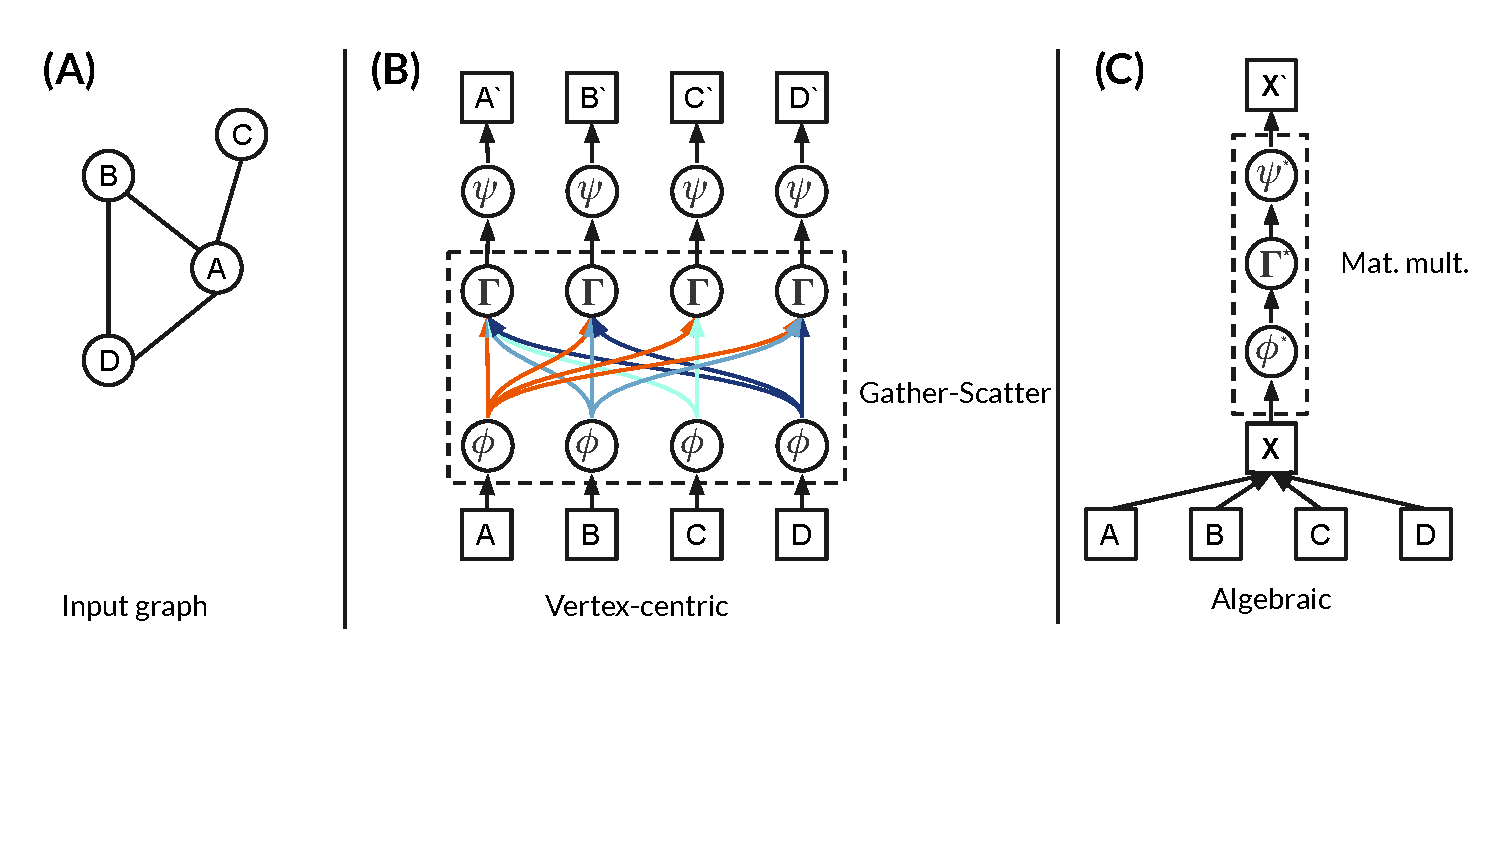
\includegraphics[width=0.70\textwidth]{./images/gnnsys.pdf}
 \caption{An example of two different approaches for GNN execution. (A): Input graph. (B): Vertex-centric approach. (C): Algebraic approach.}
 \label{fig:gnnsys}
\end{figure*}

\section{GNN Systems} \hfill \\
\label{sec:gnnsys}
So far, we have seen that GNNs are largely related to classical deep learning methods such as CNN or RNN. However, the graph data structure adds complexity as graph data can be irregular and connected explicitly. To apply to irregular data and capture a graph's structural information, various GNNs have been proposed. 

Now a natural question is: \textit{how do we build software systems to support the GNN-based graph analytics better?} And most importantly, with training/inference being the most computationally intensive part, \textit{how do we build more efficient and scalable systems for GNN training/inference}? In the past, a huge amount of effort has been put into general ML systems for classical deep learning. Most of theese are dataflow systems~\cite{spark, tf, torch}. Now it is time to consider how to re-use or develop new techniques for scalable and efficient graph deep learning. As an emerging topic, GNN system is gradually gaining popularity. 

As of now, most of the GNN system research mainly focus on the spatial methods. Majority of spatial methods can be expressed via a general update rule:
\begin{gather}
\label{eq:mp}
\mathbf{h}_v ^k = \psi ( \mathbf{x}_v^k, \gammasum_{u \in {\mathcal {N}}(v)}  \phi(\mathbf{h}_v^{k-1}, \mathbf{h}_u^{k-1}, \mathbf{x}_{e_{vu}})),
\end{gather} 
where $\psi$, $\phi$, $\Gamma$ are potentially learnable and differentiable functions, $\Gamma$ is further required to be commutative and associative. $\psi$ is called the update function, $\phi$ the message function and $\Gamma$ the aggregate function.


%\subsubsection{NeuGraph} \hfill \\
%One natural way to support GNNs in a dataflow system is to represent the GNN as a DAG and provide it to the existing system. However, it often requires loading a large amount of data into the very limited GPU memory because of the aforementioned neighbor explosion problem. And there are graph-specific optimizations that the dataflow systems would not exploit. NeuGraph~\cite{neugraph} is a system built to provide better support for GNN on top of dataflow systems.

\subsubsection{PyTorch Geometric (PyG) and NeuGraph} \hfill \\
Equation~\ref{eq:mp} fits in the paradigm of vertex-centric programming, which is a common programming model in the graph processing world~\cite{vertexcentric, powergraph, pregel} and very easy to parallelize. PyG~\cite{pyg} follows this pattern and builds GNNs as dataflow graphs on top of PyTorch~\cite{torch}, a dataflow system. Figure~\ref{fig:gnnsys} (B) shows an example computational graph generated. Each (vectorized) operation is then put on a separate processor to achieve parallelism. Built on top of PyTorch, PyG can easily utilize the features PyTorch provides, such as autograd, GPU acceleration, etc. 

NeuGraph~\cite{neugraph} is another GNN system built on top of a dataflow system and designed for a single-node multi-GPU setting. It extends the GAS~\cite{powergraph} programming model and partitions the computational graph to avoid GPU OOM issues. It further exploits GPU-to-GPU communication to avoid latencies of GPU-to-DRAM. 

\subsubsection{Deep Graph Library (DGL)} \hfill \\
DGL~\cite{dgl} takes a different approach for the GNN execution, especially for the message passing (gather-scatter) part. It takes an algebraic approach for the execution by expressing GNN as sparse matrix multiplications (SpMM). This is analogous to those algebraic approaches to general graph analytics tasks~\cite{graphla}.

Figure~\ref{fig:gnnsys} (C) gives an example of the algebraic approach taken by DGL; each step is summarized as linear algebra and executed as SpMM, which is executed via DGL's own specialized kernel. DGL is built upon existing deep learning systems, and the user can also write user-defined functions to extend the built-in functions. DGL describes itself as a framework independent system, that is, independent of the underlying deep learning system. It has full support for several popular frameworks such as Tensorflow or PyTorch as backend. Backpropagation can also be done via another SpMM, and DGL functions are registered in the underlying deep learning framework to take advantage of autograd.

The algebraic approach opens possibilities of operator fusion. For instance, consider the update rule for NN4G in Equation~\ref{eq:nn4g}, it can also be represented as Equation~\ref{eq:nn4gm} with purely matrix multiplications. Note in this form, the message function can be fused together with the aggregation function, and there is no need to materialize the intermediate messages.


\vspace{2mm}
\noindent \textbf{Comparison between PyG and DGL.} Generally speaking, the vertex-centric approach has advantages on low-degree graphs, and when the graph data is not coalesced and data access could become a bottleneck for the algebraic approaches. On the contrary, algebraic approaches do not need to materialize the huge amount of messages, leading to system crashes. Algebraic approaches could fuse the message function with the aggregation, and DGL tends to perform better on higher-degree graphs.

 

\section{Conclusion and Discussion}
\label{sec:conclusion}
In this paper, we surveyed GNN research, ranging from pioneering works to milestone papers. GNN research is gaining enormous attention, and scalability and efficiency have been one of the major topics.
We now discuss the potential research directions on the scalability and efficiency of GNNs.

On the algorithmic research of GNNs. Sampling has proven to be a very effective way of increase GNN efficiency. However, graph sampling is non-trivial because of the non-i.i.d. nature of graph data. Moreover, ignoring the interconnections may lead to degraded accuracy performance. Therefore, sophisticated sampling that considers the connections while still offering a boost in efficiency and scalability is a very important problem. Similarly, graph coarsening, which distills the original graph to be smaller subgraphs, can also significantly improve efficiency.

On the GNN system research. One natural direction for GNN system research is to scale out, i.e., distributed processing, which is receiving attention. On the other hand, they face even more problems like graph partitioning and load balancing. As mentioned before, the graph data is non-i.i.d., thus both sampling and partitioning are difficult to do. Graph partitioning for GNN itself is already a hard problem, let alone considering load-balancing simultaneously. The other important direction is compilers that can generate fused kernels for GNN operations, given a set of arbitrary user-defined functions. Such innovation would be especially useful for algebraic approaches. Meanwhile, existing general-purpose graph analytics systems may have more to offer, especially on the front of scalability and when the system needs to operate on huge graphs.


%\input{experiments}
%\input{related_work}
%\input{discussion}
%\input{acknowledgement}


% \pagebreak
\bibliography{main}
\bibliographystyle{abbrv}
%</tag>
\end{document}
